\documentclass[french,a4paper]{article}
\usepackage{lmodern}
\usepackage{amssymb,amsmath}
\usepackage{ifxetex,ifluatex}
\usepackage{fixltx2e} % provides \textsubscript
\ifnum 0\ifxetex 1\fi\ifluatex 1\fi=0 % if pdftex
  \usepackage[T1]{fontenc}
  \usepackage[utf8]{inputenc}
\else % if luatex or xelatex
  \ifxetex
    \usepackage{mathspec}
  \else
    \usepackage{fontspec}
  \fi
  \defaultfontfeatures{Ligatures=TeX,Scale=MatchLowercase}
\fi
% use upquote if available, for straight quotes in verbatim environments
\IfFileExists{upquote.sty}{\usepackage{upquote}}{}
% use microtype if available
\IfFileExists{microtype.sty}{%
\usepackage{microtype}
\UseMicrotypeSet[protrusion]{basicmath} % disable protrusion for tt fonts
}{}
\usepackage[top=2.4cm, bottom=2.1cm, outer=2cm, inner=4cm, headheight=40pt]{geometry}
\usepackage{hyperref}
\hypersetup{unicode=true,
            pdftitle={Formation aux GLM et aux modèles de distribution d'espèces},
            pdfauthor={Sébastien Rochette},
            pdfborder={0 0 0},
            breaklinks=true}
\urlstyle{same}  % don't use monospace font for urls
\ifnum 0\ifxetex 1\fi\ifluatex 1\fi=0 % if pdftex
  \usepackage[shorthands=off,main=french]{babel}
\else
  \usepackage{polyglossia}
  \setmainlanguage[]{french}
\fi
\usepackage{color}
\usepackage{fancyvrb}
\newcommand{\VerbBar}{|}
\newcommand{\VERB}{\Verb[commandchars=\\\{\}]}
\DefineVerbatimEnvironment{Highlighting}{Verbatim}{commandchars=\\\{\}}
% Add ',fontsize=\small' for more characters per line
\usepackage{framed}
\definecolor{shadecolor}{RGB}{248,248,248}
\newenvironment{Shaded}{\begin{snugshade}}{\end{snugshade}}
\newcommand{\KeywordTok}[1]{\textcolor[rgb]{0.13,0.29,0.53}{\textbf{#1}}}
\newcommand{\DataTypeTok}[1]{\textcolor[rgb]{0.13,0.29,0.53}{#1}}
\newcommand{\DecValTok}[1]{\textcolor[rgb]{0.00,0.00,0.81}{#1}}
\newcommand{\BaseNTok}[1]{\textcolor[rgb]{0.00,0.00,0.81}{#1}}
\newcommand{\FloatTok}[1]{\textcolor[rgb]{0.00,0.00,0.81}{#1}}
\newcommand{\ConstantTok}[1]{\textcolor[rgb]{0.00,0.00,0.00}{#1}}
\newcommand{\CharTok}[1]{\textcolor[rgb]{0.31,0.60,0.02}{#1}}
\newcommand{\SpecialCharTok}[1]{\textcolor[rgb]{0.00,0.00,0.00}{#1}}
\newcommand{\StringTok}[1]{\textcolor[rgb]{0.31,0.60,0.02}{#1}}
\newcommand{\VerbatimStringTok}[1]{\textcolor[rgb]{0.31,0.60,0.02}{#1}}
\newcommand{\SpecialStringTok}[1]{\textcolor[rgb]{0.31,0.60,0.02}{#1}}
\newcommand{\ImportTok}[1]{#1}
\newcommand{\CommentTok}[1]{\textcolor[rgb]{0.56,0.35,0.01}{\textit{#1}}}
\newcommand{\DocumentationTok}[1]{\textcolor[rgb]{0.56,0.35,0.01}{\textbf{\textit{#1}}}}
\newcommand{\AnnotationTok}[1]{\textcolor[rgb]{0.56,0.35,0.01}{\textbf{\textit{#1}}}}
\newcommand{\CommentVarTok}[1]{\textcolor[rgb]{0.56,0.35,0.01}{\textbf{\textit{#1}}}}
\newcommand{\OtherTok}[1]{\textcolor[rgb]{0.56,0.35,0.01}{#1}}
\newcommand{\FunctionTok}[1]{\textcolor[rgb]{0.00,0.00,0.00}{#1}}
\newcommand{\VariableTok}[1]{\textcolor[rgb]{0.00,0.00,0.00}{#1}}
\newcommand{\ControlFlowTok}[1]{\textcolor[rgb]{0.13,0.29,0.53}{\textbf{#1}}}
\newcommand{\OperatorTok}[1]{\textcolor[rgb]{0.81,0.36,0.00}{\textbf{#1}}}
\newcommand{\BuiltInTok}[1]{#1}
\newcommand{\ExtensionTok}[1]{#1}
\newcommand{\PreprocessorTok}[1]{\textcolor[rgb]{0.56,0.35,0.01}{\textit{#1}}}
\newcommand{\AttributeTok}[1]{\textcolor[rgb]{0.77,0.63,0.00}{#1}}
\newcommand{\RegionMarkerTok}[1]{#1}
\newcommand{\InformationTok}[1]{\textcolor[rgb]{0.56,0.35,0.01}{\textbf{\textit{#1}}}}
\newcommand{\WarningTok}[1]{\textcolor[rgb]{0.56,0.35,0.01}{\textbf{\textit{#1}}}}
\newcommand{\AlertTok}[1]{\textcolor[rgb]{0.94,0.16,0.16}{#1}}
\newcommand{\ErrorTok}[1]{\textcolor[rgb]{0.64,0.00,0.00}{\textbf{#1}}}
\newcommand{\NormalTok}[1]{#1}
\usepackage{longtable,booktabs}
\usepackage{graphicx,grffile}
\makeatletter
\def\maxwidth{\ifdim\Gin@nat@width>\linewidth\linewidth\else\Gin@nat@width\fi}
\def\maxheight{\ifdim\Gin@nat@height>\textheight\textheight\else\Gin@nat@height\fi}
\makeatother
% Scale images if necessary, so that they will not overflow the page
% margins by default, and it is still possible to overwrite the defaults
% using explicit options in \includegraphics[width, height, ...]{}
\setkeys{Gin}{width=\maxwidth,height=\maxheight,keepaspectratio}
\IfFileExists{parskip.sty}{%
\usepackage{parskip}
}{% else
\setlength{\parindent}{0pt}
\setlength{\parskip}{6pt plus 2pt minus 1pt}
}
\setlength{\emergencystretch}{3em}  % prevent overfull lines
\providecommand{\tightlist}{%
  \setlength{\itemsep}{0pt}\setlength{\parskip}{0pt}}
\setcounter{secnumdepth}{5}
% Redefines (sub)paragraphs to behave more like sections
\ifx\paragraph\undefined\else
\let\oldparagraph\paragraph
\renewcommand{\paragraph}[1]{\oldparagraph{#1}\mbox{}}
\fi
\ifx\subparagraph\undefined\else
\let\oldsubparagraph\subparagraph
\renewcommand{\subparagraph}[1]{\oldsubparagraph{#1}\mbox{}}
\fi

%%% Use protect on footnotes to avoid problems with footnotes in titles
\let\rmarkdownfootnote\footnote%
\def\footnote{\protect\rmarkdownfootnote}

%%% Change title format to be more compact
\usepackage{titling}

% Create subtitle command for use in maketitle
\newcommand{\subtitle}[1]{
  \posttitle{
    \begin{center}\large#1\end{center}
    }
}

\setlength{\droptitle}{-2em}
  \title{Formation aux GLM et aux modèles de distribution d'espèces}
  \pretitle{\vspace{\droptitle}\centering\huge}
  \posttitle{\par}
  \author{Sébastien Rochette}
  \preauthor{\centering\large\emph}
  \postauthor{\par}
  \predate{\centering\large\emph}
  \postdate{\par}
  \date{12 mars, 2018}

% GIS and R Course
% author : Sébastien Rochette
% contact : sebastienrochettefr@gmail.com
% website : http://statnmap.com

% \documentclass[a4paper]{article}
% Lang EN = 1, FR = 2
% \def\Lang{\Sexpr{Lang}} % 
% -- Command to find which language is loaded in babel -- %
% http://tex.stackexchange.com/questions/287667/ifpackagewith-doesnt-behave-as-i-expected-with-global-options
\usepackage{xparse}
\ExplSyntaxOn
\NewDocumentCommand{\packageoptionsTF}{mmmm}
 {
  \stanton_package_options:nnTF { #1 } { #2 } { #3 } { #4 }
 }

\cs_new_protected:Nn \stanton_package_options:nnTF
 {
  \clist_map_inline:nn { #2 }
   {
    \clist_if_in:cnTF { opt@#1.sty } { ##1 }
     { #3 } % it's a local option
     {
      \clist_if_in:cnTF { @classoptionslist } { ##1 }
       { #3 } % it's a global option
       { #4 }
     }
   }
}
\ExplSyntaxOff

% -- Define a variable depending on language -- %
\newcommand{\Lang}{0}

\makeatletter
\@ifpackageloaded{babel}{
  \packageoptionsTF{babel}{english}{%
    \renewcommand{\Lang}{1}% english
  }{%
    \renewcommand{\Lang}{2}% french
  }
}{}
\makeatother

% -- Define specific lateX options depending on language -- %
\ifnum\Lang = 1
  % \usepackage[english]{babel}
  \usepackage{enumitem}
  \setlist{itemsep = 0pt}
  \setlist{topsep = 0pt}
\fi
\ifnum\Lang = 2
  % \usepackage[french]{babel}
\fi

% --
\usepackage[utf8]{inputenc}
\usepackage[T1]{fontenc}
\usepackage{amsmath}
%\usepackage{amssymb,amsfonts,textcomp}
\usepackage{color}
\usepackage{array}
\usepackage{hhline}
%\usepackage[linktocpage=true]{hyperref} % to have only number clickable in toc
\hypersetup{linktocpage=true, colorlinks=true, linkcolor=[RGB]{241,85,34}, citecolor=[RGB]{241,85,34}, filecolor=[RGB]{241,85,34}, urlcolor=[RGB]{241,85,34}}
%\usepackage[pdftex]{graphicx}
\usepackage{tikz}
%\usepackage{float} % To force figure to be placed where I want with H
% do not use float as it changes space between figures and their caption.
% Better use [!h] option for figures
\usepackage[normalem]{ulem} % to underline text on multiple lines

\renewcommand{\emph}[1]{\textit{#1}}

\usepackage{lmodern} % For higher definition fonts
\usepackage[font = footnotesize, labelfont = bf, margin = 1cm]{caption} %name=Fig.

% Text styles
\newcommand\textstyleInternetlink[1]{\textcolor[RGB]{21,183,214}{#1}}
\newcommand\Greytext[1]{\textcolor[RGB]{75,75,75}{#1}}
\newcommand\LightGrey[1]{\textcolor[RGB]{173,169,174}{#1}}
\newcommand\OtherGrey[1]{\textcolor[RGB]{200,200,200}{#1}}


% List styles
%\newcommand\liststyleWWviiiNumii{%
%\renewcommand\labelitemi{{\textbullet}}
%\renewcommand\labelitemii{{\textbullet}}
%\renewcommand\labelitemiii{{\textbullet}}
%\renewcommand\labelitemiv{{\textbullet}}
%}

\AtBeginDocument{
\def\labelitemi{$\bullet$}%
\def\labelitemii{$\circ$}%
\def\labelitemiii{$-$}%
\def\labelitemiv{$-$}%
}

% FIGURES
% \graphicspath{{/mnt/Data/Formation_SIG-et-R/00_Original_TD_support/img_QGIS/}{/mnt/Data/Formation_SIG-et-R/00_Original_TD_support/figureR/}{/mnt/Data/Formation_SIG-et-R/00_Original_TD_support/Figures_Pres/}{/mnt/Data/autoentrepreneur/Presentation_Produits/SRochettePresentation-img/}}

%\setlength{\abovecaptionskip}{5pt}
%\setlength{\belowcaptionskip}{10pt}


% DIMENSIONS - MARGINS
% \usepackage[top=2.4cm, bottom=2.1cm, outer=2cm, inner=4cm, headheight=40pt]{geometry} %heightrounded
%\setlength\hoffset{0cm}
%\setlength\voffset{0cm}
\setlength\topmargin{-2cm}
%\setlength\headheight{2cm}
\setlength\headsep{0.50cm}
%\setlength\textheight{25.7cm}
\setlength\footskip{1.1cm}
\setlength{\parindent}{0em}
%\setlength{\parskip}{0em}
\setlength\belowcaptionskip{5pt}
\setlength\abovecaptionskip{8pt}
%\let\oldfigure\figure
%\let\oldtable\table
%\def\figure{\setlength\abovecaptionskip{5pt}\oldfigure}
%\def\table{\setlength\belowcaptionskip{1cm}\oldtable}
%\usepackage{caption} %[font = small]
%\setlength{\abovecaptionskip}{10pt plus 5pt minus 5pt}
%\captionsetup[table]{skip = 10pt}
%\captionsetup[figure]{skip = 10pt}
%\setlength\longindentation 0.60\textwidth

% \usepackage{lastpage} % to calculate number of pages to put in footer
\usepackage{pageslts}

% ----------
% BACKGROUND
% ----------
\usepackage{eso-pic}
\newcommand\BackgroundPic{%
\put(0,0){%
\parbox[b][\paperheight]{\paperwidth}{%
\vfill
\centering
  \includegraphics[width=\paperwidth,height=\paperheight]{Background_light_topdown_ThinkR.png}%
\vfill
}}}
\newcommand\BackgroundPicTitle{%
\put(0,0){%
\parbox[b][\paperheight]{\paperwidth}{%
\vfill
\centering
  \includegraphics[width=\paperwidth,height=\paperheight]{Background_Title_light_ThinkR.png}%
\vfill
}}}

%...and this immediately after \begin{document}:
%\AddToShipoutPicture*{\BackgroundPic}
%The * will make sure that the background picture will only be put on one page.
%If you wish to use the picture on multiple pages, skip the *:
%\AddToShipoutPicture{\BackgroundPic}
%Then use this command to stop using the background picture:
%\ClearShipoutPicture


% ----------
% MISE EN FORME DES TITRES
% ----------
%\renewcommand{\thesection}{\arabic{section}}
%\renewcommand{\thesubsection}{\arabic{section}.\arabic{subsection}}
%\renewcommand{\thesubsubsection}{\arabic{section}.\arabic{subsection}.\arabic{subsubsection}}

%% Provide a definition to \subparagraph to keep titlesec happy
\let\subparagraph\oldsubparagraph
\let\paragraph\oldparagraph
%% Load titlesec
%\usepackage[compact]{titlesec}
\usepackage{titlesec}
%% Revert \subparagraph to the Rmd definition
% Redefines (sub)paragraphs to behave more like sections
\ifx\paragraph\undefined\else
\let\oldparagraph\paragraph
\renewcommand{\paragraph}[1]{\oldparagraph{#1}\mbox{}}
\fi
\ifx\subparagraph\undefined\else
\let\oldsubparagraph\subparagraph
\renewcommand{\subparagraph}[1]{\oldsubparagraph{#1}\mbox{}}
\fi


%\titleformat{(command)}[(shape)]{(format)}{(label)}{(sep)}{(before)}[(after)]
\titleformat{\section}%
[block]% style du titre (block, hang, display, runin, leftmargin, drop, wrap)
{\Large\color[RGB]{21,183,214}}%changement de fonte commun au numéro et au titre
{\thesection.}% spécification du numéro
{1em}% 1em espace entre le numéro et le titre
{}% changement de fonte du titre

\titleformat{\subsection}%
[block]% style du titre (block, hang, display, runin, leftmargin, drop, wrap)
{\large\bfseries} %\itshape {\Large\bfseries\color[RGB]{30,115,190}}%changement de fonte commun au numéro et au titre
{\thesubsection.}% spécification du numéro
{1em}% {1em}% espace entre le numéro et le titre
{}% changement de fonte du titre

\titleformat{\subsubsection}%
[block]% style du titre (block, hang, display, runin, leftmargin, drop, wrap)
{\large} %\itshape {\Large\bfseries\color[RGB]{30,115,190}}%changement de fonte commun au numéro et au titre
{\thesubsubsection.}% spécification du numéro
{1em}% {1em}% espace entre le numéro et le titre
{}% changement de fonte du titre

\titleformat{\paragraph}%
[block]% style du titre (block, hang, display, runin, leftmargin, drop, wrap)
{\itshape} %\itshape {\Large\bfseries\color[RGB]{30,115,190}}%changement de fonte commun au numéro et au titre
{\theparagraph.}% spécification du numéro
{1em}% {1em}% espace entre le numéro et le titre
{}% changement de fonte du titre

\titleformat{\subparagraph}%
[block]% style du titre (block, hang, display, runin, leftmargin, drop, wrap)
{\itshape} %\itshape {\Large\bfseries\color[RGB]{30,115,190}}%changement de fonte commun au numéro et au titre
{\thesubparagraph.}% spécification du numéro
{1em}% {1em}% espace entre le numéro et le titre
{}% changement de fonte du titre


%\titlespacing*{(command)}{(left)}{(beforesep)}{(aftersep)}[(right)]
\titlespacing*{\section}{0em}{*4}{*1}

% A break for each new section with figures printed before new section
% \newcommand{\sectionbreak}{\clearpage}
% \newcommand{\sectionbreak}{\clearpage\phantomsection} % if hyperref loaded before titlesec

% Title numbering depth
\setcounter{secnumdepth}{4}
% Table of content depth
\setcounter{tocdepth}{3}
\renewcommand\contentsname{Content} % toc title


% -----------
% MISE EN FORME TEXTES SPECIAUX
% -----------
% Additionnal Text colors
\usepackage{xcolor}
\definecolor{backcolor}{RGB}{235, 235, 235}

\newcommand{\mybox}[1]{\par\noindent\colorbox{backcolor}
{\parbox{\dimexpr\textwidth-2\fboxsep\relax}{#1}}}

\newcommand{\keyword}[1]{\textcolor{red!60!black}{#1}}
\newcommand{\advert}[1]{\textit{\textcolor{orange!80!black}{#1}}}
\newcommand{\exo}[1]{\textit{\textcolor{green!80!black}{#1}}}
%\newcommand{\codecommand}[1]{\par\noindent\colorbox{backcolor}{\texttt{#1}}}
%\newcommand{\menucommand}[1]{\par\fontfamily{pcr}\fontsize{12}{12}\selectfont\color{red}\noindent\colorbox{shadecolor}{\textit{#1}}}{\par}
\newcommand{\menucommand}[1]{\textit{\textcolor{blue!80!black}{#1}}}
\newcommand{\codecommand}[1]{\texttt{\colorbox{backcolor}{#1}}}

\newenvironment{important}{\par\color{black!80!green}\itshape}{\par}

\newsavebox{\selvestebox}
\newenvironment{redbox}
  {
   \begin{lrbox}{\selvestebox}%
   \begin{minipage}{\dimexpr\columnwidth-2\fboxsep\relax}}
  {\end{minipage}\end{lrbox}%
   \colorbox[HTML]{FF7F7F}{\usebox{\selvestebox}}
   }

% \newsavebox{\selvestebox}
\newenvironment{codebox}{
  \begin{lrbox}{\selvestebox}%
}{
  \end{lrbox}%
  \colorbox{backcolor}{\usebox{\selvestebox}}
}

% - source: http://tex.stackexchange.com/questions/82028/how-do-i-create-a-variant-of-the-snugshade-box-from-the-framed-package-to-wrap-m
\newenvironment{blueShaded}[1][D6E8F5]{
  \definecolor{shadecolor}{HTML}{#1}%
  \begin{snugshade}%
}{%
    \end{snugshade}%
}

% -- command for pandoc trick with \begin and \end -- %
\newcommand{\nopandoc}[1]{#1}

% ----------
% Pour justifier le texte apres un alignement à gauche
% Utile pour le texte en caractère tt qui ne se coupe pas
% ----------
\usepackage{ragged2e}

% \input{/mnt/Data/ThinkR/Gitlab/vignette-thinkr/latex/MiseEnFormeTitreFormationRmd_NoSectionBreak.tex}

\ifnum\Lang = 1
% ---------------
% HEADER / FOOTER
% ---------------
\usepackage{fancyhdr}
\pagestyle{fancy}
%\fancyhf{}
\fancyhead[L]{
\hspace{-1cm}\LARGE{\textbf{\href{https://thinkr.fr/}{ThinkR}}}\\
%\hspace{-1cm}\normalsize{\Greytext{Modélisation statistique, analyse de données géographiques et cartographie}}\\
\hspace{-1cm}\normalsize{\Greytext{Courses and consulting for R}}\\
%\normalsize{\href{url:http://statnmap.com/}{\textstyleInternetlink{http://statnmap.com/}}}
}
\fancyhead[R]{\Greytext{\textit{Created on \today}\hspace{-1cm}}}
%
\fancyfoot[L]{\Greytext{\hspace{-1cm}Sébastien Rochette}}
\fancyfoot[C]{\href{mailto:sebastien@thinkr.fr}{sebastien@thinkr.fr}}
\fancyfoot[R]{\Greytext{\thepage\ / \pageref*{LastPage}\hspace{-1cm}}}
%\cfoot{Page \thepage\ (\theCurrentPage) of \lastpageref{LastPages}}
\renewcommand{\headrulewidth}{0pt}
\renewcommand{\footrulewidth}{0pt}
%\fancyheadoffset{length}


\fi
\ifnum\Lang = 2
% ---------------
% HEADER / FOOTER
% ---------------
\usepackage{fancyhdr}
\pagestyle{fancy}
%\fancyhf{}
\fancyhead[L]{
\hspace{-1cm}\LARGE{\textbf{\href{https://thinkr.fr/}{ThinkR}}}\\
%\hspace{-1cm}\normalsize{\Greytext{Modélisation statistique, analyse de données géographiques et cartographie}}\\
\hspace{-1cm}\normalsize{\Greytext{Formation et consultance sur R}}\\
%\normalsize{\href{url:http://sebrock.fr/}{\textstyleInternetlink{http://sebrock.fr/}}}
}
\fancyhead[R]{\Greytext{\textit{Créé le \today}\hspace{-1cm}}}
%
\fancyfoot[L]{\Greytext{\hspace{-1cm}Sébastien Rochette}}
\fancyfoot[C]{\href{mailto:sebastien@thinkr.fr}{sebastien@thinkr.fr}}
% \fancyfoot[R]{\Greytext{\thepage\ / \pageref*{LastPage}\hspace{-1cm}}}
%\cfoot{Page \thepage\ (\theCurrentPage) of \lastpageref{LastPages}}
\fancyfoot[R]{\Greytext{\thepage\ / \pageref*{LastPage}\hspace{-1cm}}}
\renewcommand{\headrulewidth}{0pt}
\renewcommand{\footrulewidth}{0pt}
%\fancyheadoffset{length}

\fi

% -- Graphic path -- %
% \graphicspath{{/mnt/Data/Formation_SIG-et-R/00_Original_TD_support/img_QGIS/}{/mnt/Data/Formation_SIG-et-R/00_Original_TD_support/figureR/}{/mnt/Data/Formation_SIG-et-R/00_Original_TD_support/Figures_Pres/}{/mnt/Data/autoentrepreneur/Presentation_Produits/SRochettePresentation-img/}}
\graphicspath{{/mnt/Data/ThinkR/Gitlab/vignette-thinkr/img/}}

% \title{GIS and R Course}
% \author{Sébastien Rochette}

\setcounter{section}{0} % Value for first section


\hypersetup{pdfauthor=Sébastien Rochette, pdftitle=Formation ThinkR, pdfsubject=Formation à R, pdfkeywords=R, pdfcreator=pdflatex}

%----------------------------------------------------------------------------------------
% TITLE PAGE
%----------------------------------------------------------------------------------------

\newcommand*{\titleGM}{\begingroup % Create the command for including the title page in the document
\hbox{ % Horizontal box
%\hspace*{0.2\textwidth} % Whitespace to the left of the title page
%\hspace*{0.2\textwidth}
\OtherGrey{\rule{1pt}{\textheight}} % Vertical line
\hspace*{0.05\textwidth} % Whitespace between the vertical line and title page text
\parbox[b]{0.75\textwidth}{ % Paragraph box which restricts text to less than the width of the page

{\noindent\Huge\bfseries\textstyleInternetlink{ Formation à R}}\\[2\baselineskip] % Title
{\large{Modélisation avec les GLM}}\\[4\baselineskip] % Tagline or further description
{\Large \textsc{Sébastien Rochette, ThinkR}} % Author name

\vspace{0.5\textheight} % Whitespace between the title block and the publisher
{\noindent \href{url:https://thinkr.fr}{ThinkR}}\\[\baselineskip] % Publisher and logo
}}
\endgroup}

\AtBeginDocument{\let\maketitle\relax}

\begin{document}
\maketitle

\pagenumbering{arabic}

%\bigskip
%\medskip

%\begin{center}
%\href{url:http://statnmap.com}{\textstyleInternetlink{\huge{Modelling distribution of species in the Bay of Biscay}}}\\
%\large{Sébastien Rochette}\\
%\end{center}
\setcounter{page}{0}
\pagestyle{empty} % Removes page numbers
\AddToShipoutPicture{\BackgroundPicTitle}

\titleGM

\pagebreak
\pagestyle{fancy}
% \clearpage\setcounter{page}{1}\pagestyle{Standard}
\AddToShipoutPicture{\BackgroundPic}

{
\setcounter{tocdepth}{2}
\tableofcontents
}
\section{Préface}\label{preface}

\emph{La version d'origine de cette formation a été créée par Olivier Le
Pape et Étienne Rivot à Agrocampus Ouest (Rennes, France). Depuis mon
doctorat dans leur équipe, je mets à jour constamment cette formation au
gré de ma recherche et de l'évolution du logiciel R.}

\begin{Shaded}
\begin{Highlighting}[]
  \CommentTok{# Generated with R and rmarkdown: Roadmap version - Teacher}
\end{Highlighting}
\end{Shaded}

\section{Présentation de l'étude}\label{presentation-de-letude}

\textbf{\advert{Le contexte et les objectifs de votre étude définissent le type de modélisation que vous allez mettre en place sur votre jeu de données.}\\
Ici, nous utilisons les modèles linéaires généralisés pour produire une
carte de distribution moyenne de la nourricerie de soles communes de la
baie de Vilaine}.

\subsection{Contexte}\label{contexte}

\begin{itemize}
\tightlist
\item
  Les zones côtières et les estuaires sont des habitats halieutiques
  essentiels

  \begin{itemize}
  \tightlist
  \item
    Zones à forte production
  \item
    Nourriceries
  \item
    Zones restreintes avec de fortes densités (Fig.
    \ref{fig:figPlaiceBox})
  \end{itemize}
\end{itemize}



\begin{figure}[!h]

{\centering 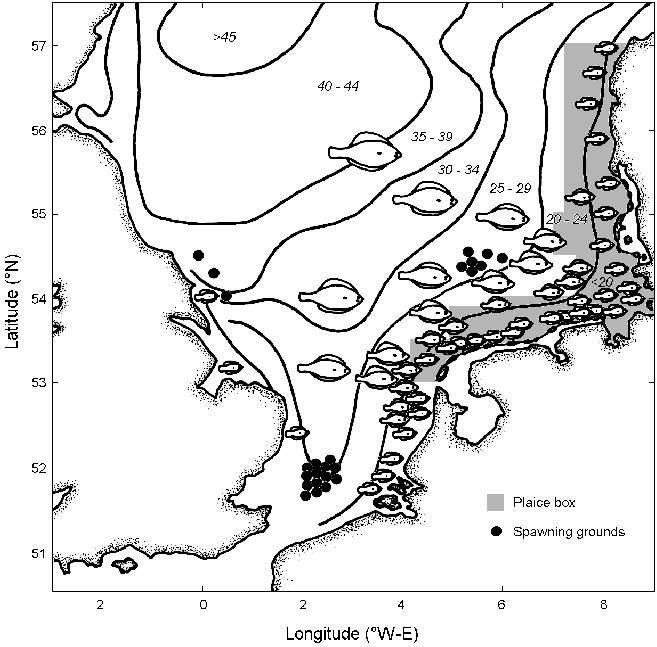
\includegraphics[width=0.5\linewidth]{/mnt/Data/ThinkR/Gitlab/formation-glm/03_Figures/00_Presentation/PlaiceBox_crop} 

}

\caption{Plaice box (Rijnsdorp \emph{et al.})}\label{fig:figPlaiceBox}
\end{figure}

\begin{itemize}
\tightlist
\item
  Pression anthropique élevée

  \begin{itemize}
  \tightlist
  \item
    Perte de surface disponibles (Fig. \ref{fig:figHighPressure}a)
  \item
    Qualité des habitats alterée (Fig. \ref{fig:figHighPressure}b)
  \end{itemize}
\end{itemize}




\begin{itemize}
\tightlist
\item
  Impact sur le renouvellement des populations

  \begin{itemize}
  \tightlist
  \item
    Jeune stades = Gouleau d'étranglement
  \item
    La taille et la qualité des nourriceries côtières influent sur la
    production de juvéniles
  \end{itemize}
\end{itemize}

\begin{figure}[!h]

{\centering 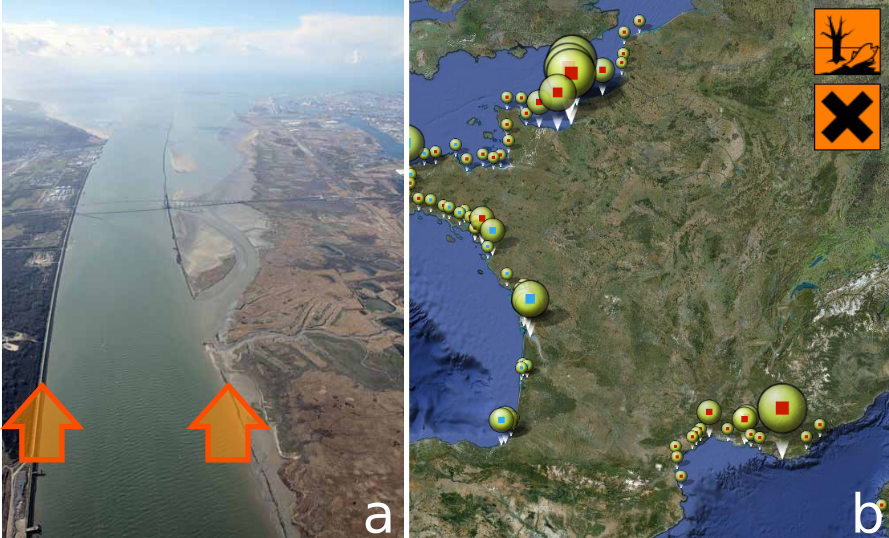
\includegraphics[width=0.8\linewidth]{/mnt/Data/ThinkR/Gitlab/formation-glm/03_Figures/00_Presentation/HighPressure} 

}

\caption{(a) L'estuaire de la Seine. (b) Niveau de
contamination chimique le long des côtes françaises (Ifremer, 2011)}\label{fig:figHighPressure}
\end{figure}

\subsection{Objectifs}\label{objectifs}

Déterminer les facteurs ayant une influence sur la distribution des
poissons plats (\emph{Solea solea}) en Baie de Vilaine et cartographier
la distribution moyenne des densités.

\begin{itemize}
\tightlist
\item
  Cartographier les habitats potentiels nécessite:

  \begin{itemize}
  \tightlist
  \item
    Connaissance des habitats de juvéniles
  \item
    Campagnes d'échantillonnage dans la zone d'étude
  \item
    Connaissance des covariables environnementales ayant potentiellement
    de l'influence

    \begin{itemize}
    \tightlist
    \item
      Cartes exhaustives des covariables environnementales
    \end{itemize}
  \end{itemize}
\item
  Une approche statistique en deux étapes

  \begin{itemize}
  \tightlist
  \item
    Modèle statistique reliant les densités aux covariables
  \item
    Prédire les habitats potentiels
  \end{itemize}
\end{itemize}

\subsection{Données}\label{donnees}

Campagne standardisée de chalut à perche dans la baie de Vilaine (Fig.
\ref{fig:figVilaineCampaign})

\begin{itemize}
\tightlist
\item
  1984 -- 2010
\item
  En autumne
\item
  Juvéniles de l'année (Âge 0)

  \begin{itemize}
  \tightlist
  \item
    Nb individus / 1000m\textsuperscript{2}
  \end{itemize}
\end{itemize}




\begin{figure}[!h]

{\centering 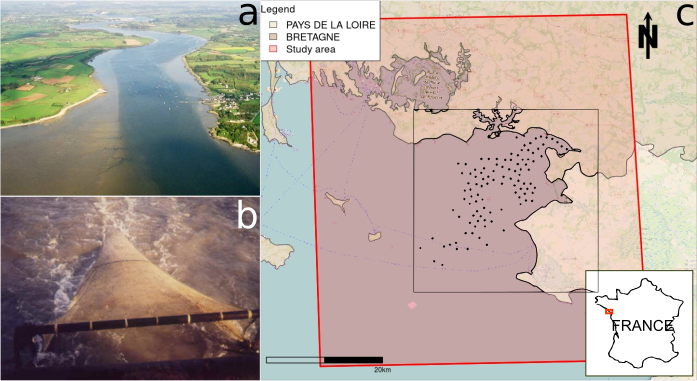
\includegraphics[width=0.8\linewidth]{/mnt/Data/ThinkR/Gitlab/formation-glm/03_Figures/00_Presentation/Vilaine_Campaign} 

}

\caption{(a) L'estuaire de la Vilaine. (b) Chalut à
perche. (c) Situation des stations d'échantillonnage.}\label{fig:figVilaineCampaign}
\end{figure}

\subsection{Covariables}\label{covariables}

\begin{itemize}
\tightlist
\item
  Bathymétrie (Fig. \ref{fig:figCovariates}a)

  \begin{itemize}
  \tightlist
  \item
    MNT à 1000m de résolution
  \item
    Projection Mercator
  \end{itemize}
\item
  Structure sédimentainre (Fig. \ref{fig:figCovariates}b)

  \begin{itemize}
  \tightlist
  \item
    Fichier shape de polygones
  \item
    Coordonnées géographiques
  \end{itemize}
\item
  Zones biologiques (Fig. \ref{fig:figCovariates}c)

  \begin{itemize}
  \tightlist
  \item
    Combinaison bathymétrie, sédiment, habitat
  \item
    Fichier shape de polygones
  \item
    Coordonnées géographiques
  \end{itemize}
\end{itemize}




\begin{figure}[!h]

{\centering 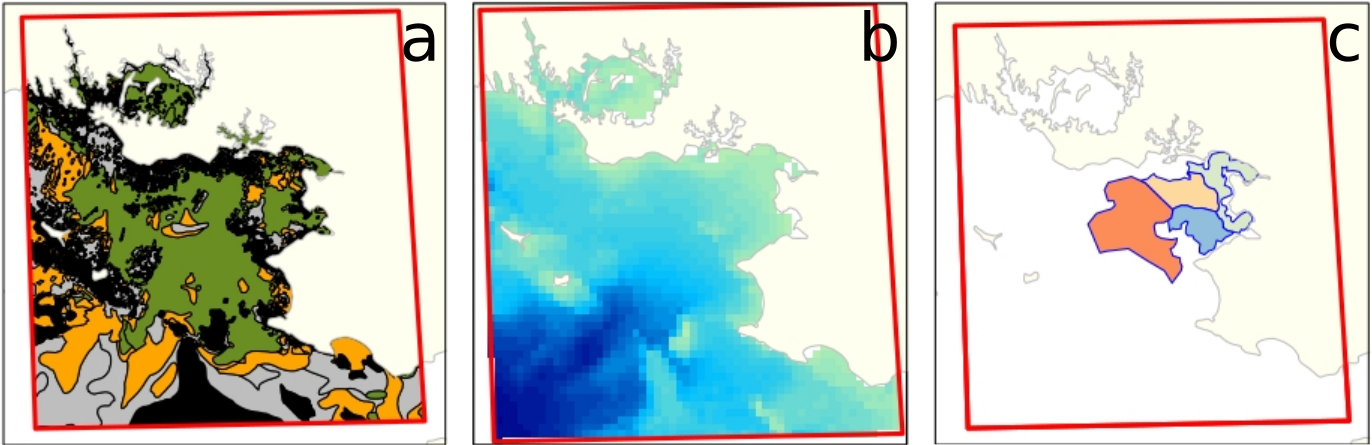
\includegraphics[width=0.8\linewidth]{/mnt/Data/ThinkR/Gitlab/formation-glm/03_Figures/00_Presentation/Day2-02Vilaine-Covariates_abc} 

}

\caption{Covariables en baie de Vilaine. (a) Structure
sédimentaire, (b) Bathymétrie et (c) Zones biologiques.}\label{fig:figCovariates}
\end{figure}

\subsection{Ajuster un modèle de distribution
d'espèces}\label{ajuster-un-modele-de-distribution-despeces}

\begin{itemize}
\tightlist
\item
  Croiser les données avec les cartes de covariables

  \begin{itemize}
  \tightlist
  \item
    Utiliser un modèle linéaire
  \end{itemize}
\item
  Utiliser les cartes des covariables pour la prédiction (Fig.
  \ref{fig:figProcedure})

  \begin{itemize}
  \tightlist
  \item
    Une prédiction pour chaque cellule d'un raster
  \end{itemize}
\end{itemize}



\begin{figure}[!h]

{\centering 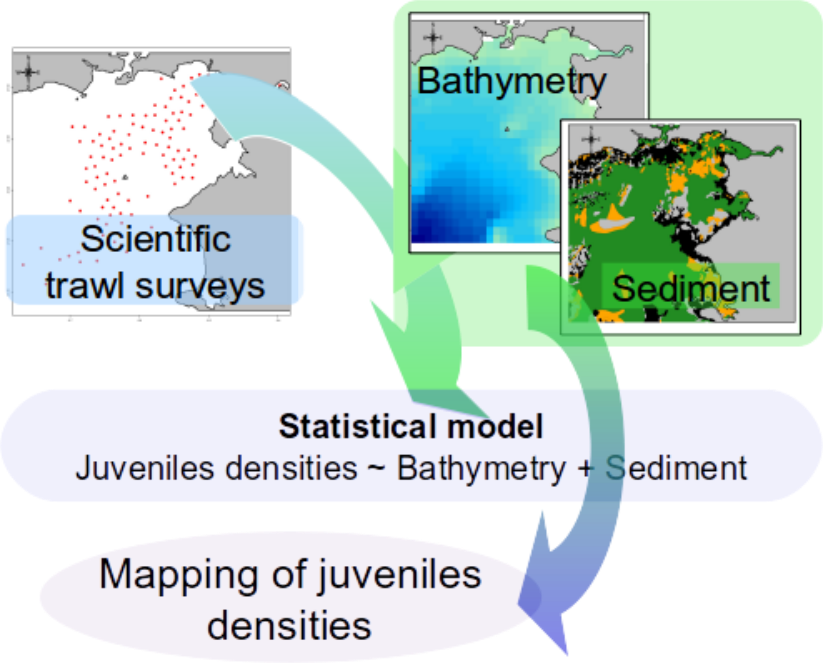
\includegraphics[width=0.7\linewidth]{/mnt/Data/ThinkR/Gitlab/formation-glm/03_Figures/00_Presentation/Schema_Modele} 

}

\caption{Procédure pour un modèle de distribution d'espèce}\label{fig:figProcedure}
\end{figure}

\subsection{Exploration des données}\label{exploration-des-donnees}

\nopandoc{\begin{redbox}} Prenez le temps d'explorer vos données avant
toutes analyses \nopandoc{\end{redbox}}

\begin{itemize}
\tightlist
\item
  Explorer les données et les covariables

  \begin{itemize}
  \tightlist
  \item
    Explorer le plan d'échantillonnage
  \item
    Explorer les liens potentiels entre les densités et les covariables
  \item
    Explorer les futurs paramètres de modélisation (interactions,
    distributions)
  \end{itemize}
\end{itemize}

\advert{Souvenez-vous toujours des objectifs de votre étude !}

\exo{Question : Que recherchons-nous dans cette exploration ?}

\section{Préparation}\label{preparation}

\subsection{Structure des dossiers}\label{structure-des-dossiers}

\advert{Il convient de toujours conserver les fichiers originaux : les reprojections entraînent toujours quelques pertes, mieux vaut revenir aux originaux lorsque c'est possible.}

L'arborescence de votre dossier de travail est la suivante :

\begin{itemize}
\tightlist
\item
  \includegraphics[width=0.26in]{/mnt/Data/ThinkR/Gitlab/vignette-thinkr/img/icon-folder_Blue_12px}
  01\_Original\_data

  \begin{itemize}
  \tightlist
  \item
    \includegraphics[width=0.26in]{/mnt/Data/ThinkR/Gitlab/vignette-thinkr/img/icon-folder_Blue_12px}
    DEPARTEMENTS
  \item
    \includegraphics[width=0.26in]{/mnt/Data/ThinkR/Gitlab/vignette-thinkr/img/icon-folder_Blue_12px}
    Sedim\_GDG\_wgs84
  \item
    \includegraphics[width=0.26in]{/mnt/Data/ThinkR/Gitlab/vignette-thinkr/img/icon-file_Blue_12px}
    bathy\_GDG\_1000\_merc (and co)
  \item
    \includegraphics[width=0.26in]{/mnt/Data/ThinkR/Gitlab/vignette-thinkr/img/icon-file_Blue_12px}
    Data\_Vilaine\_solea.csv
  \end{itemize}
\item
  \includegraphics[width=0.26in]{/mnt/Data/ThinkR/Gitlab/vignette-thinkr/img/icon-folder_Blue_12px}
  02\_Outputs
\item
  \includegraphics[width=0.26in]{/mnt/Data/ThinkR/Gitlab/vignette-thinkr/img/icon-folder_Blue_12px}
  03\_Figures
\item
  \includegraphics[width=0.26in]{/mnt/Data/ThinkR/Gitlab/vignette-thinkr/img/icon-folder_Blue_12px}
  04\_Functions
\end{itemize}

\subsection{Débutons avec R}\label{debutons-avec-r}

\begin{itemize}
\tightlist
\item
  Créer un projet Rstudio dans le dossier principal de travail.
\item
  Ouvrez le script R : ``Quick\_AllDataModel\_Teacher.R''
\item
  Lister les différents sous-dossier de travail au début de votre script
  R
\end{itemize}

\begin{Shaded}
\begin{Highlighting}[]
\CommentTok{# Define working directories ---------------------------------------------------}
\NormalTok{WD <-}\StringTok{ }\KeywordTok{here}\NormalTok{()}
\CommentTok{# Folder of original files}
\NormalTok{origWD <-}\StringTok{ }\KeywordTok{here}\NormalTok{(}\StringTok{"01_Original_data"}\NormalTok{)}
\CommentTok{# Folder for outputs}
\NormalTok{saveWD <-}\StringTok{ }\KeywordTok{here}\NormalTok{(}\StringTok{"02_Outputs"}\NormalTok{)}
\CommentTok{# Folder where to save outputs from R}
\NormalTok{figWD <-}\StringTok{ }\KeywordTok{here}\NormalTok{(}\StringTok{"03_Figures"}\NormalTok{)}
\CommentTok{# Folder where complementary functions are stored}
\NormalTok{funcWD <-}\StringTok{ }\KeywordTok{here}\NormalTok{(}\StringTok{"04_Functions"}\NormalTok{)}
\end{Highlighting}
\end{Shaded}

\section{Exploration des données}\label{exploration-des-donnees-1}

\subsection{Étapes}\label{etapes}

\advert{Souvenez-vous : Définissez ce que vous cherchez, à quelles questions vous souhaiteriez répondre !}

\begin{itemize}
\tightlist
\item
  Explorer la répartition du plan d'échantillonnage en fonction des
  covariables environementales
\item
  Explorer les données d'observation au regard des covariables
  environnementales pour détecter de potentielles corrélations
\item
  Explorer les interactions entre les effets des covariables sur les
  observations
\item
  Explorer les lois de distribution possibles (gaussian, log-normal,
  \ldots{}) des observations en fonctions des combinaisons de
  covariables \nopandoc{\begin{redbox}} Les scripts qui sont fournis ne
  sont que des exemples, ils ne sont en aucun cas les meilleures
  solutions ! Faîtes vos propres tests ! \nopandoc{\end{redbox}}
\end{itemize}

\subsection{Liste des différentes
étapes}\label{liste-des-differentes-etapes}

\begin{itemize}
\tightlist
\item
  Lire le jeu de données spatialisé (Fig. \ref{fig:RFigDataGG})
\end{itemize}



\begin{figure}[!h]

{\centering 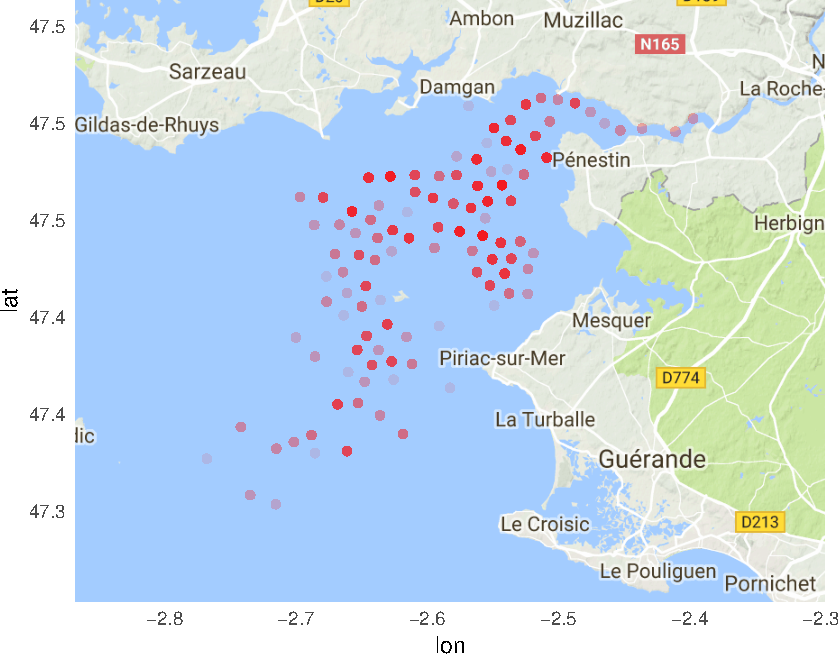
\includegraphics[width=0.9\linewidth]{FR_Quick_AllDataModel_Teacher_files/figure-latex/RFigDataGG-1} 

}

\caption{Répartition des stations d'échantillonnage}\label{fig:RFigDataGG}
\end{figure}

\begin{itemize}
\tightlist
\item
  Ajouter une nouvelle covariable : la bathymétrie divisée en classes

  \begin{itemize}
  \tightlist
  \item
    " \textless{} 5 m``,''5-10 m``,''10-20 m``,''20-50 m"
  \end{itemize}
\item
  Explorer la répartition des observations en fonctions des covariables

  \begin{itemize}
  \tightlist
  \item
    Centrer l'analyse sur l'année, la bathymétrie et le sédiment
  \item
    \exo{Que remarquez-vous ?}
  \end{itemize}
\item
  Explorer les covariables ayant potentiellement des effets sur les
  densités

  \begin{itemize}
  \tightlist
  \item
    \exo{Quelles covariables pourraient avoir une influence ?}(Fig.
    \ref{fig:RFigHistGG})
  \end{itemize}
\end{itemize}




\begin{figure}[!h]

{\centering 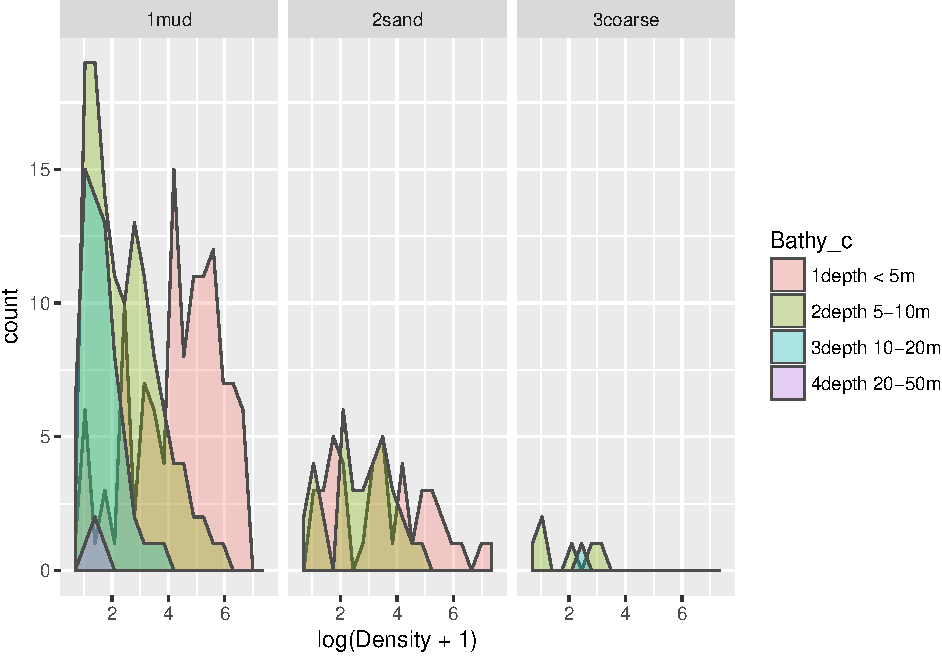
\includegraphics[width=1\linewidth]{FR_Quick_AllDataModel_Teacher_files/figure-latex/RFigHistGG-1} 

}

\caption{Densités (log-transformées) en fonction de la
bathymétrie et des sédiments}\label{fig:RFigHistGG}
\end{figure}

Les modèles statistiques que nous allons utiliser peuvent se résumer de
cette façon : \[Density = Covar1 + Covar2 + Noise\] Comme vous le savez,
on chercher toujours à savoir si les données sont gaussienne pour
pouvoir procéder à l'analyse statistique. Si elles ne sont pas
gaussienne, nous devons définir le type de distribution pour pouvoir
utiliser une transformation de données.

\begin{itemize}
\tightlist
\item
  Explorer la distribution des données
\item
  \exo{Quelle est la distribution la plus intéressante ?}
\end{itemize}

La figure \ref{fig:RFigDistrib} montre différents exemples de
distributions.



\begin{figure}[!h]

{\centering 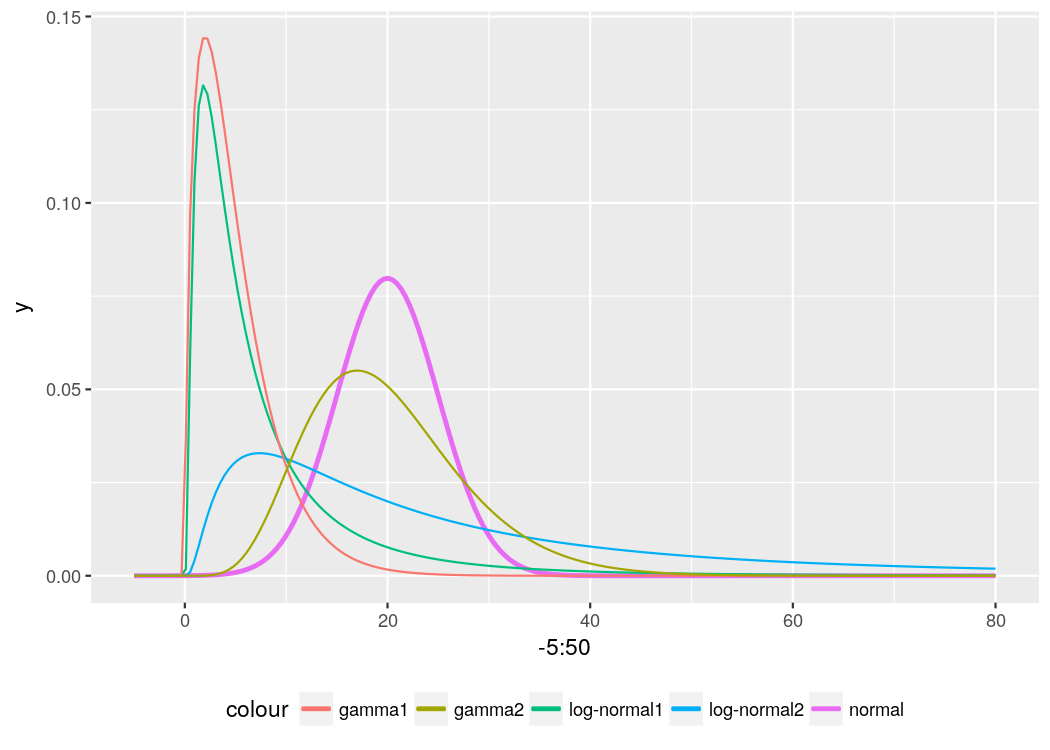
\includegraphics[width=0.9\linewidth]{FR_Quick_AllDataModel_Teacher_files/figure-latex/RFigDistrib-1} 

}

\caption{Différents exemples de distributions\\}\label{fig:RFigDistrib}
\end{figure}

Exemple de l'effet de deux facteurs (Fig. \ref{fig:RFigTwoFact})



\begin{itemize}
\tightlist
\item
  \exo{Qu'en pensez-vous ?}
\end{itemize}

\begin{figure}[!h]

{\centering 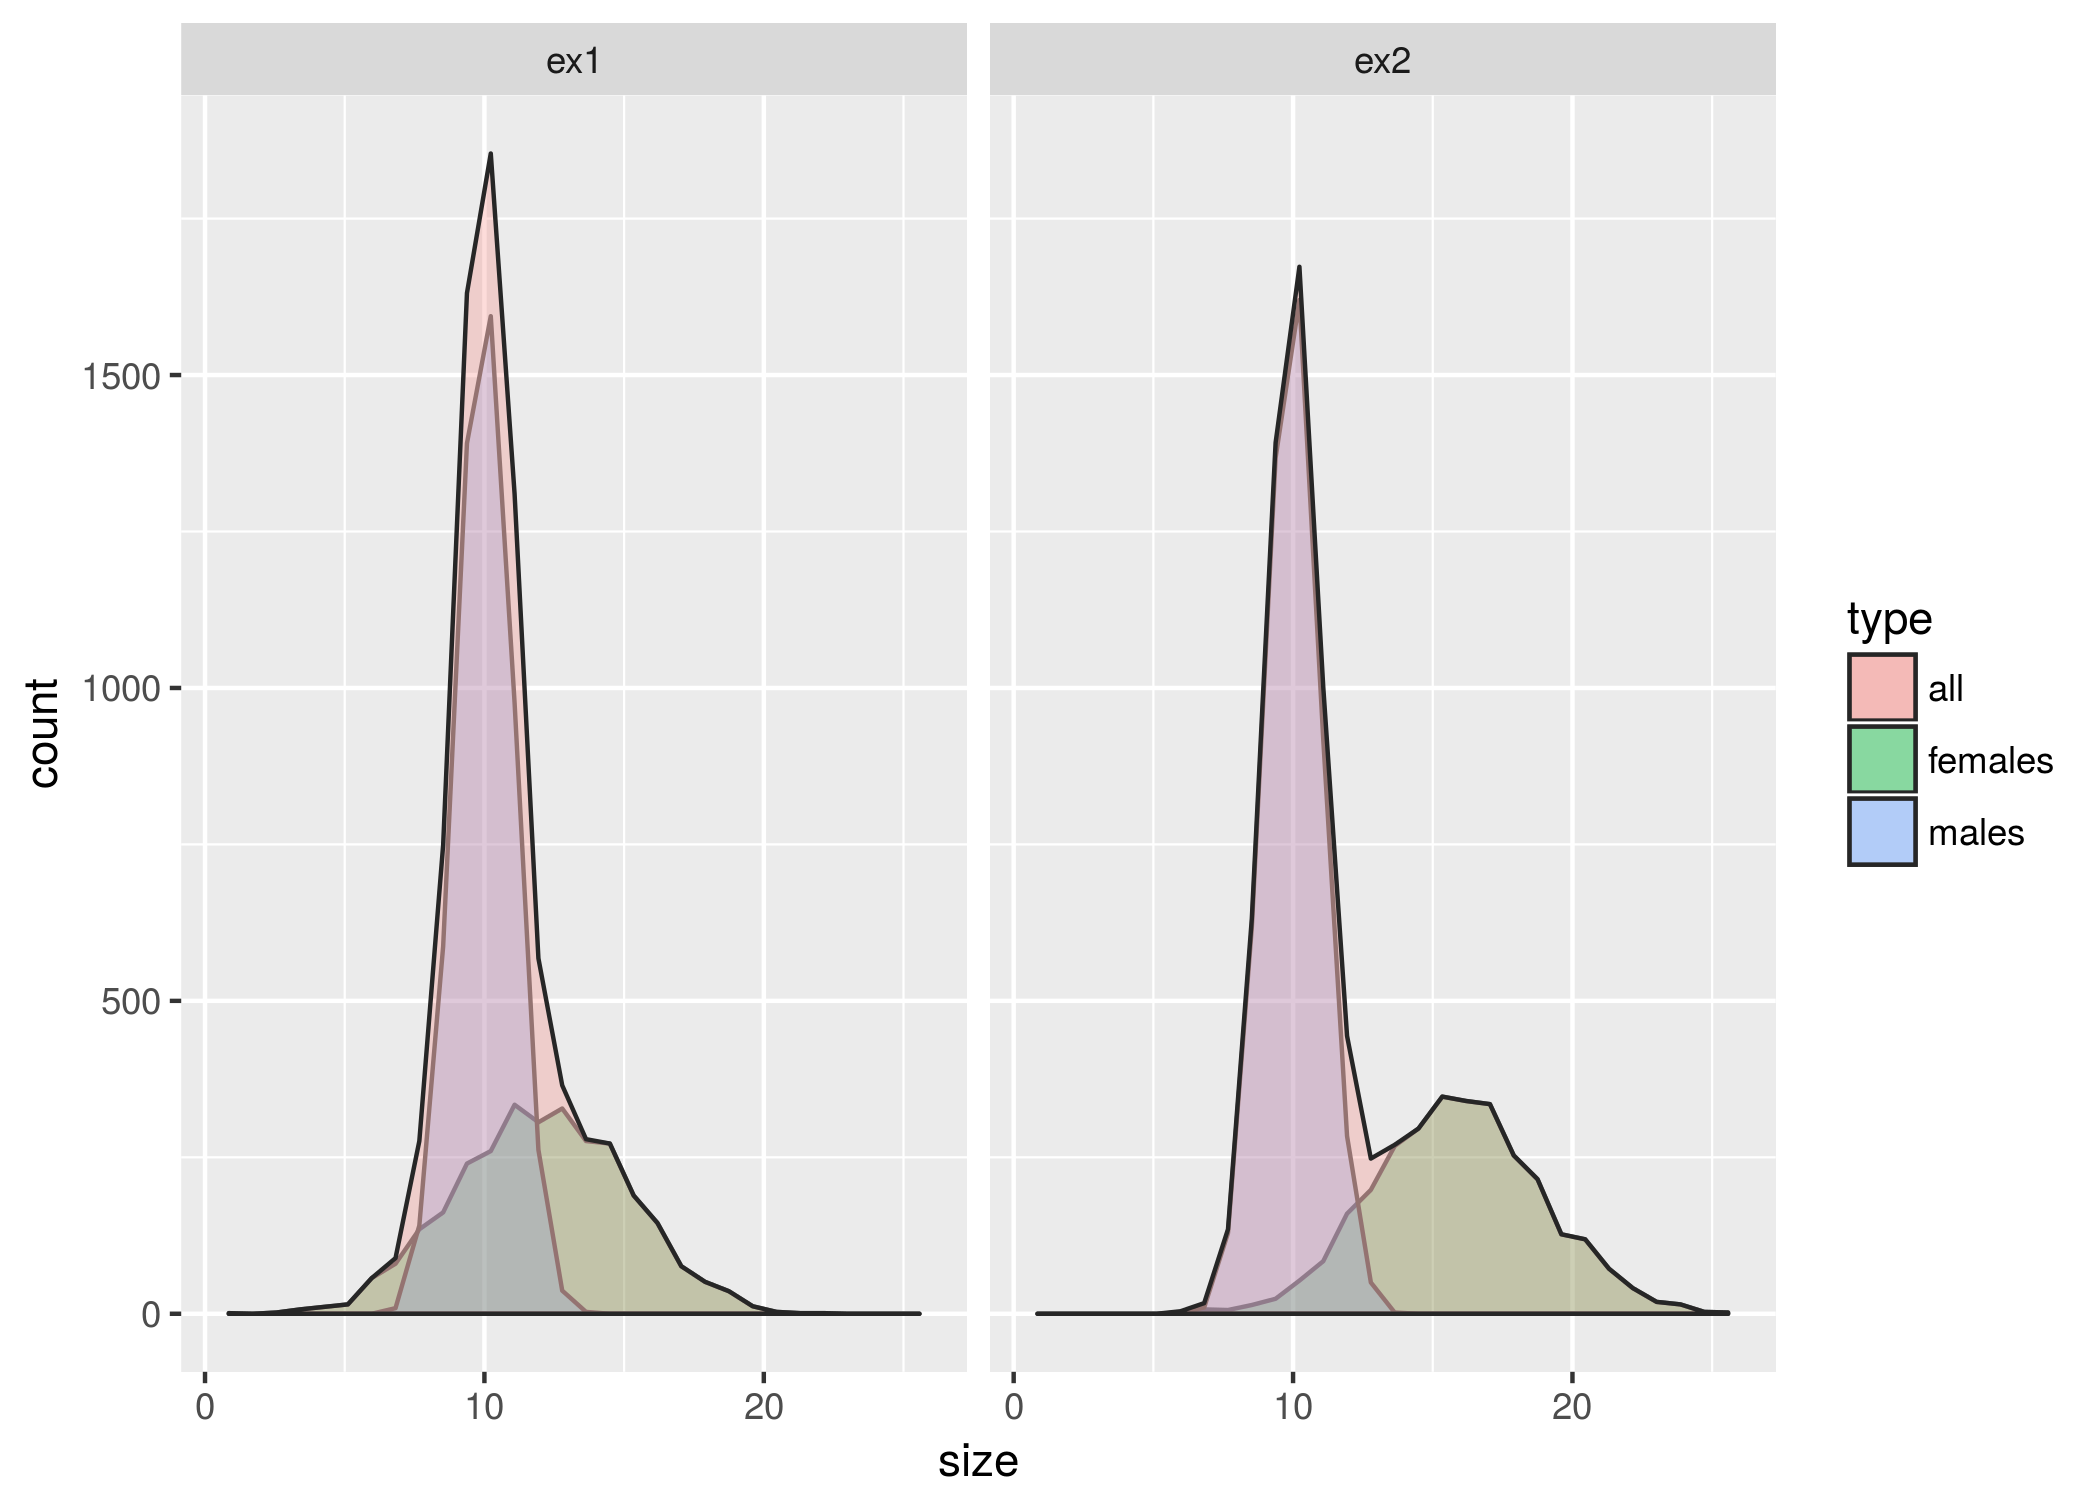
\includegraphics[width=1\linewidth]{FR_Quick_AllDataModel_Teacher_files/figure-latex/RFigTwoFact-1} 

}

\caption{Differents effets de deux facteurs}\label{fig:RFigTwoFact}
\end{figure}

\begin{itemize}
\tightlist
\item
  Explorer les interactions potentielles entre les covariables

  \begin{itemize}
  \item
    \exo{Qu'en pensez-vous ?}
  \item
    Comme aide à l'interprétation, utiliser l'exemple théorique de la
    figure \ref{fig:RFigExInteractions}
  \end{itemize}
\end{itemize}



\begin{figure}[!h]

{\centering 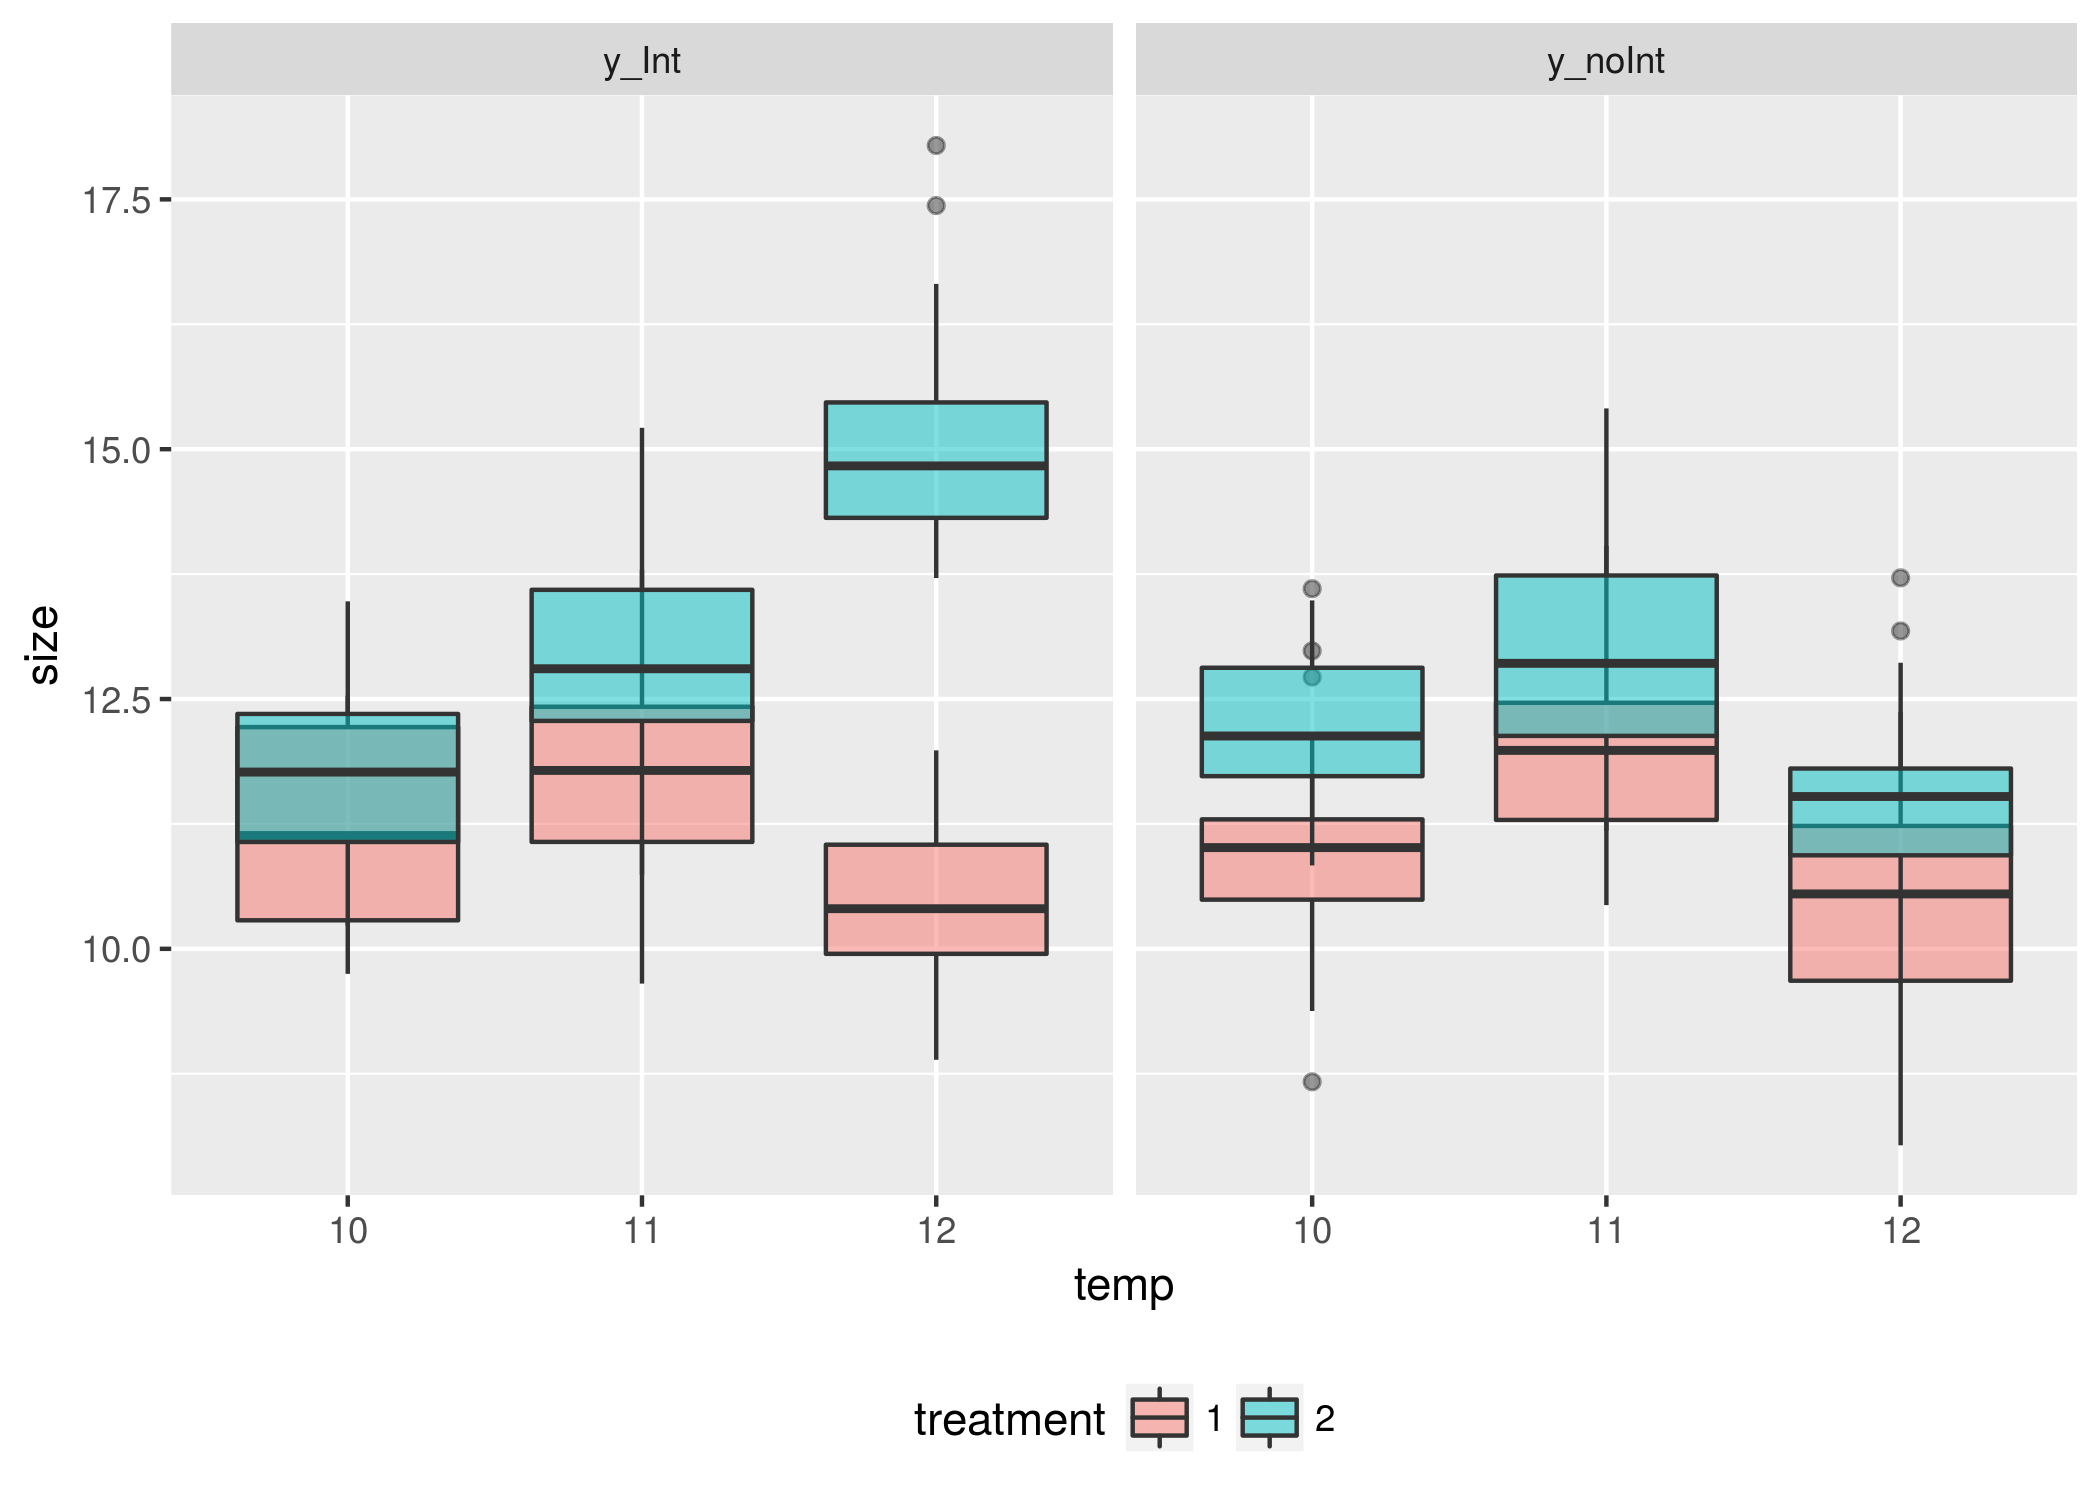
\includegraphics[width=0.8\linewidth]{FR_Quick_AllDataModel_Teacher_files/figure-latex/RFigExInteractions-1} 

}

\caption{Interaction entre traitements et température}\label{fig:RFigExInteractions}
\end{figure}

\section{Modélisation}\label{modelisation}

\subsection{Étapes}\label{etapes-1}

\advert{Souvenez-vous: Définissez ce que vous cherchez, à quelles questions vous souhaiteriez répondre !}

\begin{itemize}
\tightlist
\item
  Tester les différentes formes de modèles au regard des combinaisons de
  covariables et des formes de distributions des résidus
\item
  Comparer les modèles à l'aide des outils statistiques à disposition
  (AIC, anova, \ldots{}), de la validation croisée mais aussi de la
  connaissance du jeu de données et des questions ciblées
\item
  Analyser les résidus des modèles. Analyser leur distribution et
  s'assurer que les hypothèses de construction sont vérifiées.\\
  \advert{C'est seulement lorsque les hypothèses sur la distribution des résidus sont vérifiées, que les covariables et les interactions sélectionnées peuvent commencer à être interprétées...}
  \nopandoc{\begin{redbox}} Les scripts qui sont fournis ne sont que des
  exemples, ils ne sont en aucun cas les meilleures solutions ! Faîtes
  vos propres tests ! \nopandoc{\end{redbox}}
\end{itemize}

\subsection{Interpréter les sorties de
modèles}\label{interpreter-les-sorties-de-modeles}

Lorsque vous ajustez un modèle linéaire (lm ou glm), vous pouvez
utiliser différents tests statistiques et visuels qui répondent à
différentes questions. Votre question principale pourrait être :

\begin{itemize}
\tightlist
\item
  ``Est-ce que mes covariables ont un effet sur mes observations ?''. En
  réalité, ce n'est pas exactement la question à laquelle va répondre
  votre modèle. Ce serait plutôt ``Est-ce que les covariables que j'ai
  utilisées expliquent une part de la variabilité de mes observations
  ?''
\end{itemize}

Pour que vous puissiez interpréter les différentes sorties de modèles,
dans ce document, nous allons regarder le modèle suivant :
\[lm(Density ~ Bathy + Sedim, data = dataset)\] \emph{Ce modèle n'est
pas forcément le meilleur modèle à choisir !}

\subsubsection{Summary(lm)}\label{summarylm}

Cette fonction montre un tableau de tests de significativité (Table
\ref{tab:RTableSummary}). Ce sont des tests de Student. Ils testent si
la valeur estimée pour un effet est ou non significativement différente
de zéro. Ainsi, si une covariable a un effet non significativement
différent de l'effet nul, il est probablement inutile de la conserver
dans le modèle.

\begin{itemize}
\tightlist
\item
  Ici, ce qui est appelé ``Intercept'' est l'effet de base. Dans une
  équation \(y = a.x + b\), l'``intercept'' serait \(b\). Ici, c'est un
  peu différent car il y a des covariables au format facteur
  (``Sedim''). Dans cet exemple, l'``intercept'' montre une ``p-value''
  proche de zéro, ce qui signifie que son effet
  (\texttt{estimate\ \textasciitilde{}\ 100}) est significativement
  différent de zéro.
\item
  La covariable ``Bathy'' est continue. Dans une équation de type
  \(y = a.x + b\) ce serait \(a\). Dans cet exemple, son effet
  \texttt{estimate\ \textasciitilde{}\ 6}, est significativement
  différent de zéro (\texttt{p-value\ \textasciitilde{}\ 0}).
\item
  La covariable ``Sedim'' est un facteur à trois niveaux. Dans le
  ``summary'', vous ne pouvez en voir que deux (``2sand'', ``3coarse'').
  En réalité, les effets des niveaux de facteur (\(estimate\)) sont
  comparés au premier niveau (``1mud''), pour lequel l'effet est égal à
  zéro. Dans l'équation \(Y = a*Bathy + b[Sedim] + c\), l'estimation de
  la moyenne Y pour \texttt{Sedim\ =\ "1mud"} est
  \(Y = a*Bathy + 0 + c\). Dans les résultats du tableau,
  \texttt{b{[}"2sand"{]}} est donc non significativement différent de
  \texttt{b{[}"1mud"{]}\ =\ 0}, et, \texttt{b{[}"3coarse"{]}} avec une
  \texttt{p-value\ =\ 0.07}, n'est pas non plus significativement
  différent de \texttt{b{[}"1mud"{]}\ =\ 0}.
\end{itemize}

\begin{table}

\caption{\label{tab:RTableSummary}Exemple d'une sortie de `summary(lm)`}
\centering
\begin{tabular}[t]{l|r|r|r|r}
\hline
  & Estimate & Std. Error & t value & Pr(>|t|)\\
\hline
(Intercept) & 173.4 & 14.27 & 12.152 & 0.000\\
\hline
Bathy & 14.5 & 1.71 & 8.472 & 0.000\\
\hline
Sedim2sand & -19.5 & 19.07 & -1.020 & 0.308\\
\hline
Sedim3coarse & -39.4 & 57.21 & -0.689 & 0.491\\
\hline
\end{tabular}
\end{table}

\subsubsection{Analyse de résidus}\label{analyse-de-residus}

Une hypothèse de construction d'un modèle linéaire est
l'homoscédasticité, aussi appelée homogénéité de la variance. Cela
signifie que la variance de la réponse \texttt{y} est la même quelque
soit la valeur du prédicteur \texttt{x}. Dans un modèle Gaussien
classique ajustant \texttt{x} à \texttt{y} ainsi:
\(y = a.x + b + \epsilon\), la variable \(\epsilon\) représente les
résidus du modèle. Ils sont supposés être centrés sur zéro et avec une
variance Gaussienne, leur distribution suivant ainsi la loi Gaussienne
\(\epsilon \sim N(0, \sigma)\)\\
Lorsqu'on simule un tel modèle, par exemple \(y = 2.x + 5 + \epsilon\),
on observe la figure \ref{fig:RFigResidualsExemple}, avec une
homogénéité de la distribution des observations autour de l'ajustement,
et une distribution Gaussienne des résidus comme le montrent
l'histogramme et le ``qqplot''.




\begin{Shaded}
\begin{Highlighting}[]
\CommentTok{# Example of homogeneous residuals}
\NormalTok{n <-}\StringTok{ }\DecValTok{1000}
\NormalTok{epsilon <-}\StringTok{ }\KeywordTok{rnorm}\NormalTok{(n, }\DecValTok{0}\NormalTok{, }\DecValTok{5}\NormalTok{)}
\NormalTok{x <-}\StringTok{ }\KeywordTok{runif}\NormalTok{(n, }\DecValTok{0}\NormalTok{, }\DecValTok{10}\NormalTok{)}
\NormalTok{y <-}\StringTok{ }\DecValTok{2}\OperatorTok{*}\NormalTok{x }\OperatorTok{+}\StringTok{ }\DecValTok{5} \OperatorTok{+}\StringTok{ }\NormalTok{epsilon}

\KeywordTok{par}\NormalTok{(}\DataTypeTok{mfrow =} \KeywordTok{c}\NormalTok{(}\DecValTok{1}\NormalTok{,}\DecValTok{3}\NormalTok{))}
\KeywordTok{plot}\NormalTok{(x, y, }\DataTypeTok{pch =} \DecValTok{20}\NormalTok{)}
\KeywordTok{abline}\NormalTok{(}\DecValTok{5}\NormalTok{, }\DecValTok{2}\NormalTok{, }\DataTypeTok{col =} \StringTok{"red"}\NormalTok{, }\DataTypeTok{lwd =} \DecValTok{2}\NormalTok{)}
\KeywordTok{hist}\NormalTok{(epsilon, }\DataTypeTok{breaks =} \DecValTok{20}\NormalTok{, }\DataTypeTok{col =} \StringTok{"grey"}\NormalTok{)}
\KeywordTok{qqnorm}\NormalTok{(epsilon); }\KeywordTok{qqline}\NormalTok{(epsilon, }\DataTypeTok{col =} \StringTok{"red"}\NormalTok{)}
\end{Highlighting}
\end{Shaded}

\begin{figure}[!h]

{\centering 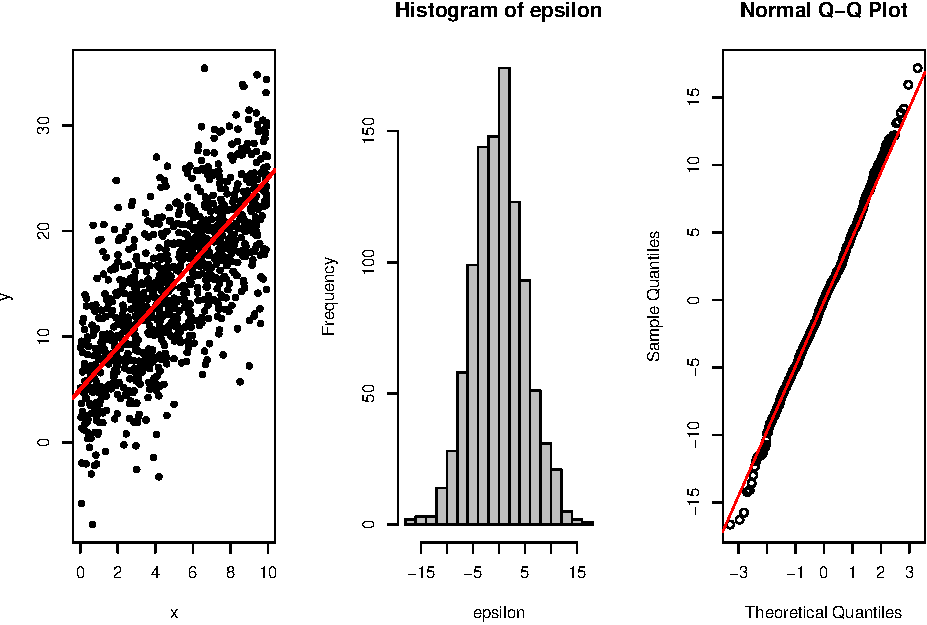
\includegraphics{FR_Quick_AllDataModel_Teacher_files/figure-latex/RFigResidualsExemple-1} 

}

\caption{Simulation d'une relation linéaire entre x
et y avec un résidu Gaussien.}\label{fig:RFigResidualsExemple}
\end{figure}

À partir de cet exemple, vous pouvez définir les diagnostics graphiques
nécessaires pour vérifier vos hypothèses de construction de modèle.
Lorsqu'on utilise le même modèle que précédemment
(Fig.\ref{fig:RFigResidualsDiag}) :

\begin{itemize}
\tightlist
\item
  \texttt{Residuals\ vs\ Fitted} - Dans cet exemple, on peut voir que la
  variablité des résidus augmente avec les valeurs prédites, ce qui va à
  l'encontre de l'homogénéité de la variance.
\item
  \texttt{Scale-Location} est en accord avec la figure précédente car on
  voit une augmentation de la deviance des résidus quand les prédictions
  augmentent.
\item
  \texttt{Normal\ Q-Q} - Cette figure appelée ``qqplot'' montre la
  divergence entre les quantiles théoriques d'une loi Gaussienne et les
  quantiles réels de la distribution des résidus du modèle. La
  divergence est importante pour les valeurs élevées, ce qui montre une
  queue de distribution plus longue qu'une loi Normale.
\item
  \texttt{Hist.\ of\ residuals} - L'histogramme des résidus est en
  accord avec le qqplot car on voit clairement un distribution qui n'est
  pas une Gaussienne centrée sur zéro. Cette distribution a une longue
  queue de distribution avec beaucoup plus de valeurs positives que de
  valeurs négatives.
\end{itemize}




\begin{figure}[!h]

{\centering 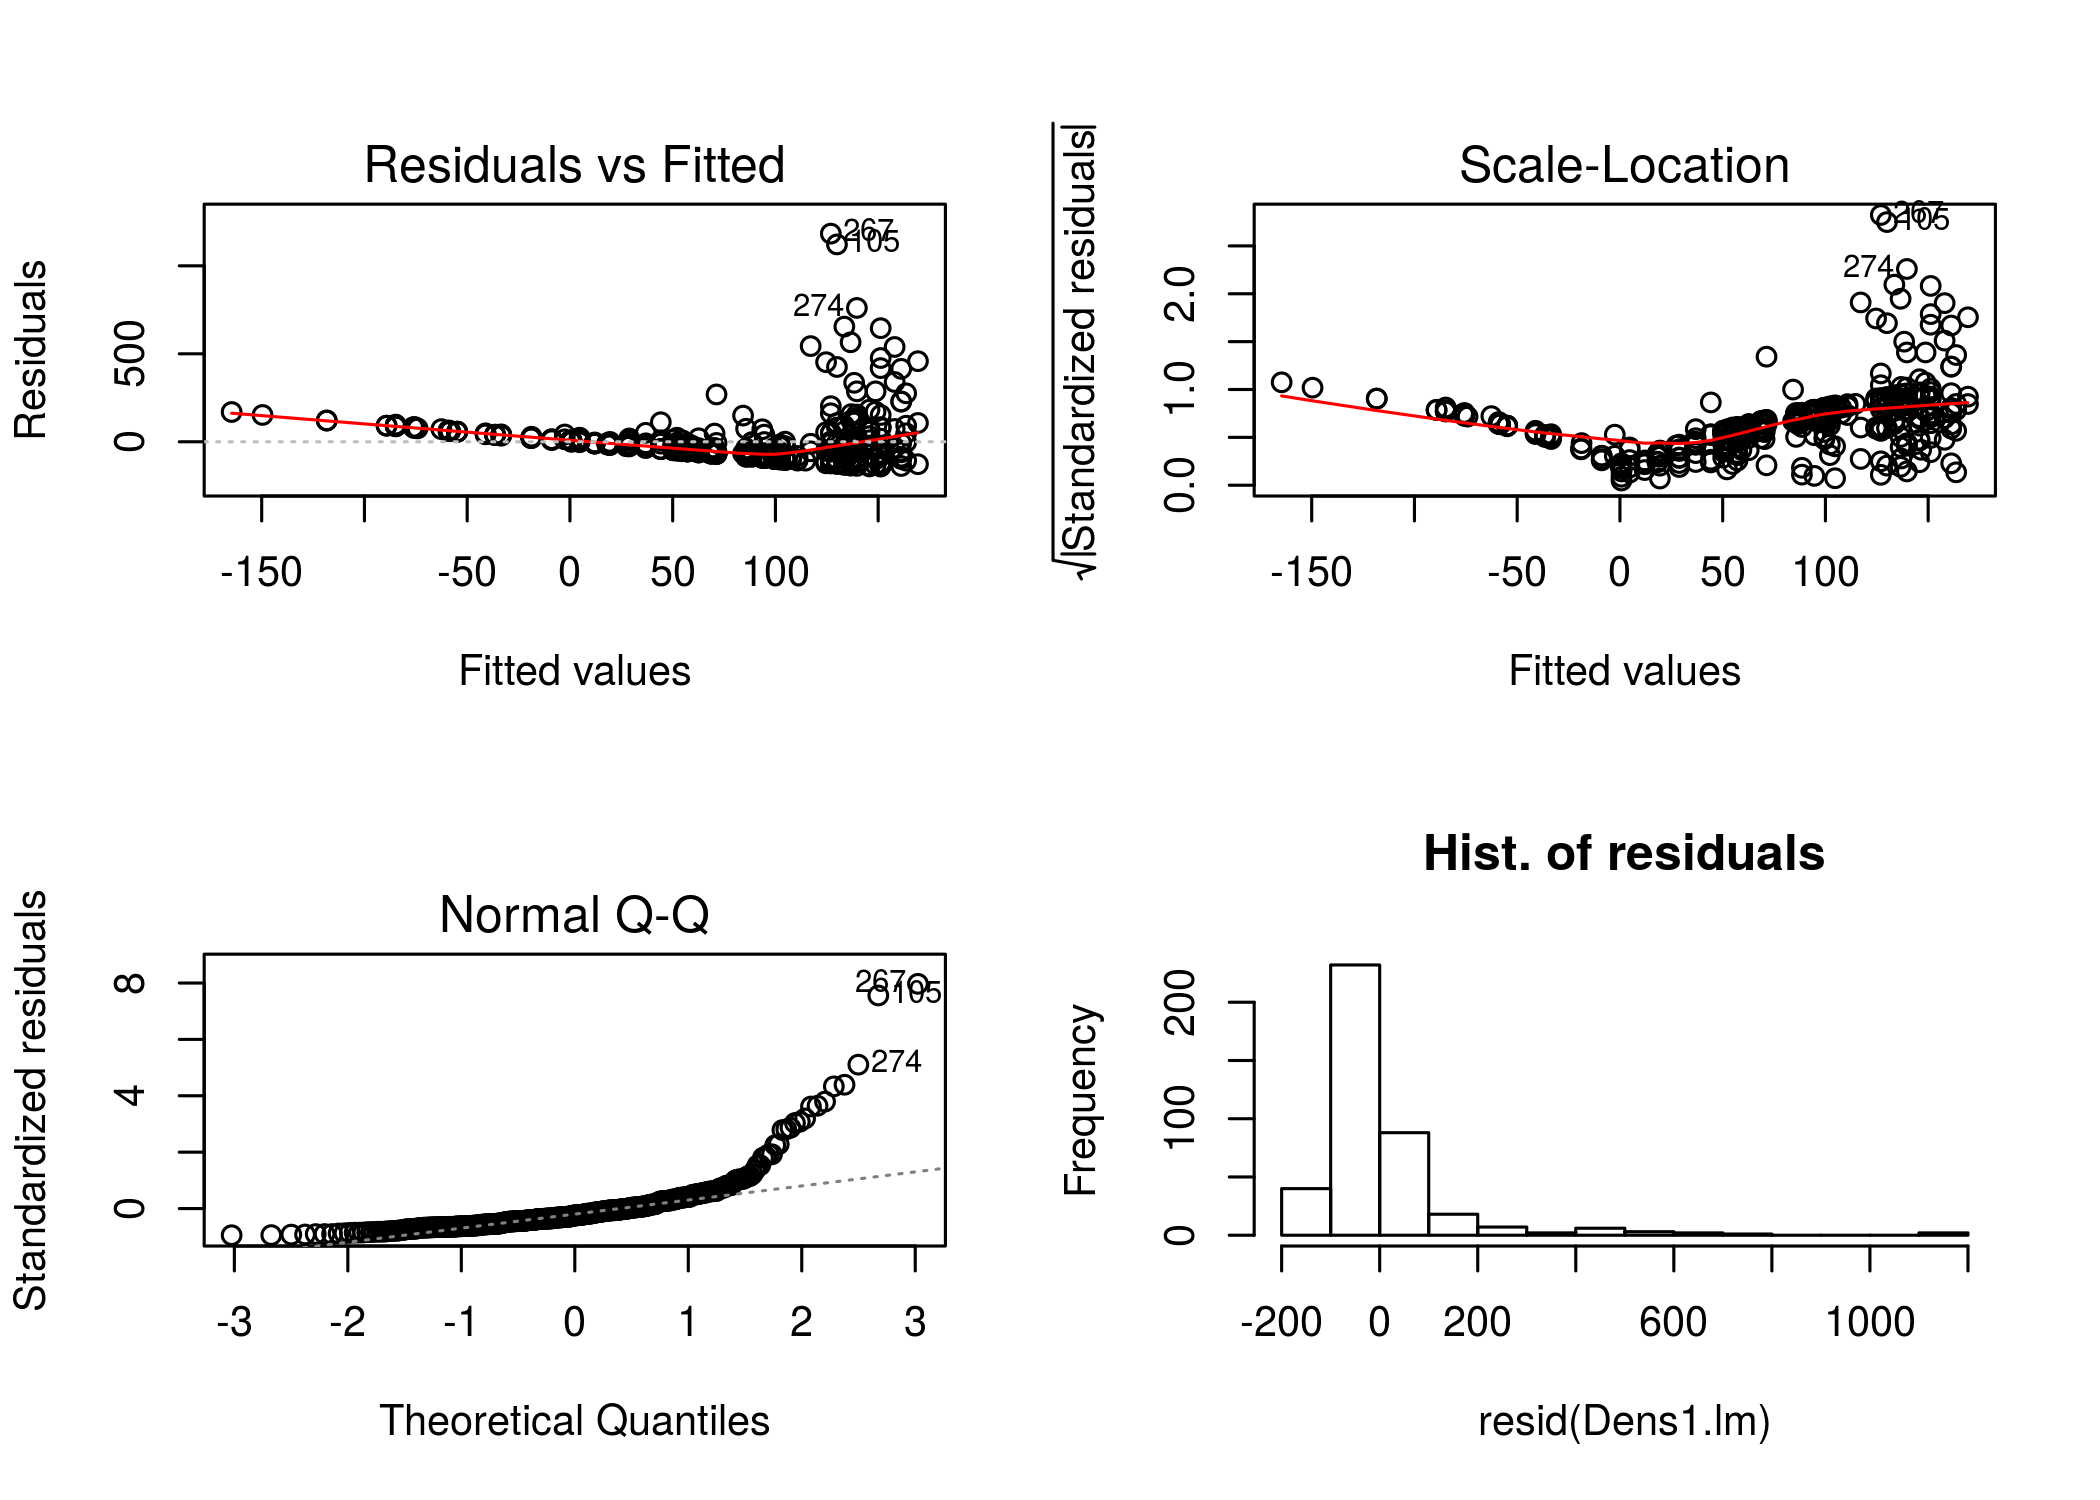
\includegraphics{FR_Quick_AllDataModel_Teacher_files/figure-latex/RFigResidualsDiag-1} 

}

\caption{Figures de diagnostic d'un modèle linéaire
permettant de vérifier les hypothèses de construction.}\label{fig:RFigResidualsDiag}
\end{figure}

\subsubsection{Analyse de variance}\label{analyse-de-variance}

La question à laquelle répond une \texttt{anova} (avec un test du Chi-2)
est : Est-ce que la covariable ajoutée augmente significativitement la
vraisemblance du modèle (ou a réduit la déviance résiduelle), comparé au
modèle précédent, sans cette covariable ?

\begin{itemize}
\tightlist
\item
  \texttt{NULL} est le test pour un modèle sans covariable, c'est le
  modèle qui estime la moyenne : \(Density \sim constant\).
\item
  \texttt{Bathy} est le test pour un modèle uniquement avec la
  \texttt{Bathy} : \(Density \sim Bathy\). La \texttt{p-value} est
  proche de zéro, indiquant que le gain de déviance expliquée en
  ajoutant la \texttt{Bathy} est significativement différent de zéro.
\item
  \texttt{Sedim} est le test pour un modèle avec \texttt{Bathy} et
  \texttt{Sedim}, dans cet ordre : \(Density \sim Bathy + Sedim\). La
  \texttt{p-value\ \textasciitilde{}\ 0.2} indique qu'il y a un risque
  de 20\% que la déviance expliquée en ajoutant la covariable
  \texttt{Sedim} au modèle contenant déjà la \texttt{Bathy} soit nulle.
\end{itemize}

\begin{table}

\caption{\label{tab:RTableAnova}Exemple d'une `sortie` de anova(lm)}
\centering
\begin{tabular}[t]{l|r|r|r|r|r}
\hline
  & Df & Sum Sq & Mean Sq & F value & Pr(>F)\\
\hline
Bathy & 1 & 1607692 & 1607692 & 71.983 & 0.000\\
\hline
Sedim & 2 & 32206 & 16103 & 0.721 & 0.487\\
\hline
Residuals & 397 & 8866764 & 22334 & NA & NA\\
\hline
\end{tabular}
\end{table}

\subsubsection{Critères d'Akaike (AIC) et Bayesian
(BIC)}\label{criteres-dakaike-aic-et-bayesian-bic}

L'AIC et le BIC sont des critères de qualité d'ajustement pénalisés par
le nombre de paramètres estimés. La description (traduite) de ces
fonctions dans R est :

\begin{quote}
Function générique calculant ``Le Critère d'Information'' d'Akaike pour
un ou plusieurs modèles ajustés pour lesquels une ``log-vraisemblance''
peut être obtenue, en utilisant la formule
\(IC = -2*log-likelihood + k*npar\), où \texttt{npar} represente le
nombre de paramètres estimés, et \texttt{k\ =\ 2} pour l'AIC classique,
ou \texttt{k\ =\ log(n)} (\texttt{n} étant le nombre d'observations)
pour le BIC ou SBC (Schwarz's Bayesian criterion).
\end{quote}

En effet, plus vous ajoutez de paramètres dans un modèle, plu svous avez
de chances que le modèle s'ajuste parfaitement aux données (Table
\ref{tab:RTableAnovaEx}, Fig. \ref{fig:RFigAICExample}). L'AIC diminue
avec la déviance résiduelle et augmente avec le nombre de paramètres
ajustés. Plus l'AIC est bas, plus parsimonieux est le modèle.




\begin{table}

\caption{\label{tab:RTableAnovaEx}Comparaison de la déviance expliquée par différents modèles avec un nombre croissant de paramètres}
\centering
\begin{tabular}[t]{l|r|r|r|r|r|l|r|r}
\hline
model & Res.Df & RSS & Df & Sum of Sq & Pr(>Chi) & "||" & df & AIC\\
\hline
lm1 & 8 & 3192 & NA & NA & NA & || & 3 & 92.0\\
\hline
lm2 & 6 & 1272 & 2 & 1920 & 0.003 & || & 5 & 86.8\\
\hline
lm3 & 4 & 645 & 2 & 626 & 0.144 & || & 7 & 84.1\\
\hline
\end{tabular}
\end{table}

\begin{figure}[!h]

{\centering 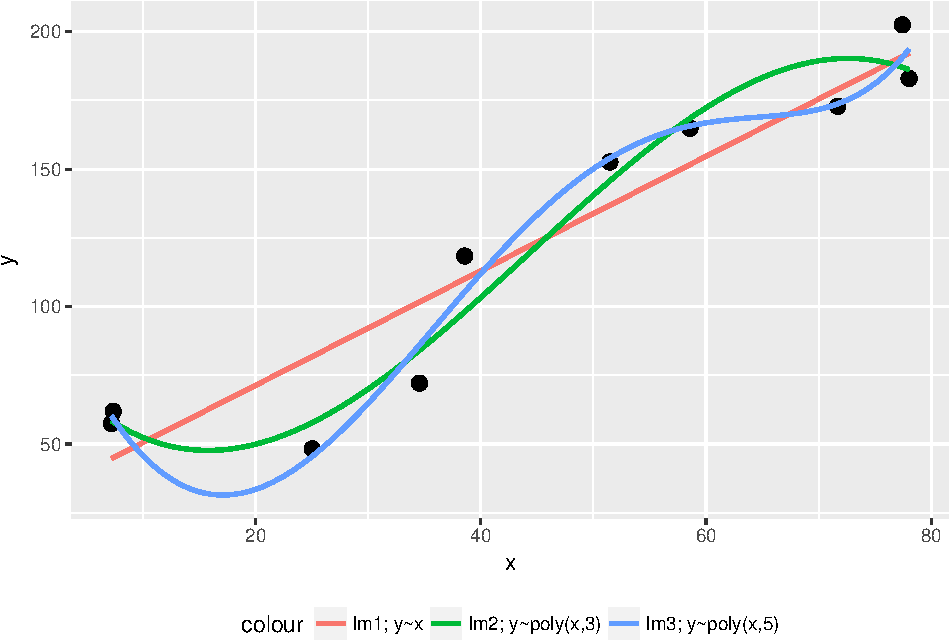
\includegraphics{FR_Quick_AllDataModel_Teacher_files/figure-latex/RFigAICExample-1} 

}

\caption{Différents modèles ajustés sur les mêmes données
mais avec un nombre de paramètres ajustés croissant.}\label{fig:RFigAICExample}
\end{figure}

\subsection{Trouver le meilleur
modèle}\label{trouver-le-meilleur-modele}

La fonction \codecommand{lm} n'est utilisée que pour des modèles avec
une distribution Gaussienne des résidus. Pour tester d'autres types de
distributions, il faut utiliser \codecommand{glm}, avec un paramètre
pour la famille de distribution (\codecommand{family}). Vous pouvez
utiliser des distributions qui autorisent une plus grande queue de
distribution que la loi Normale. Parmis les familles disponibles, vous
pouvez tester \codecommand{poisson, quasipoisson, Gamma, Log-gaussian}.

\begin{itemize}
\tightlist
\item
  \exo{Quel est le meilleur modèle au regard des différents critères évoqués ?}
\end{itemize}

\subsubsection{Exploration des sorties du meilleur
modèle}\label{exploration-des-sorties-du-meilleur-modele}

\begin{itemize}
\tightlist
\item
  \exo{Que pouvez-vous dire sur le diagnostic complet de votre modèle ?}
  (Fig. \ref{fig:RFigGLMResults})
\end{itemize}



\begin{figure}[!h]

{\centering 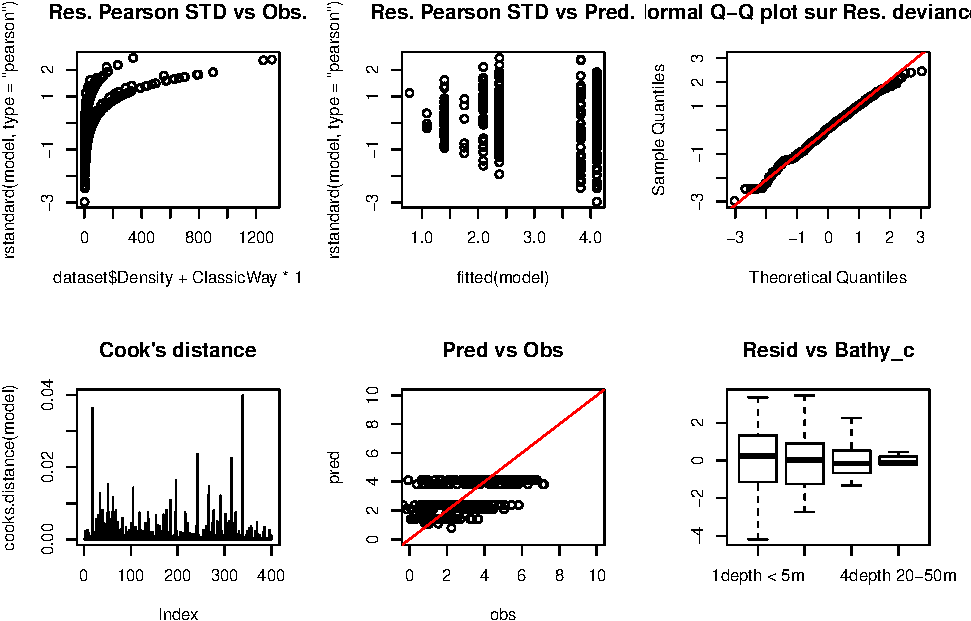
\includegraphics{FR_Quick_AllDataModel_Teacher_files/figure-latex/RFigGLMResults-1} 

}

\caption{Diagnostic du meilleur GLM sélectionné}\label{fig:RFigGLMResults}
\end{figure}

\subsection{Prédictions du modèle}\label{predictions-du-modele}

Lorsque vous êtes satisfaits du modèle sélectionné, vous pouvez faire
des prédictions

\begin{itemize}
\tightlist
\item
  Utiliser le fichier csv fourni pour voir l'effet des covariables
  sélectionnées (Fig. \ref{fig:RFigGLMPredict})
\end{itemize}



\begin{figure}[!h]

{\centering 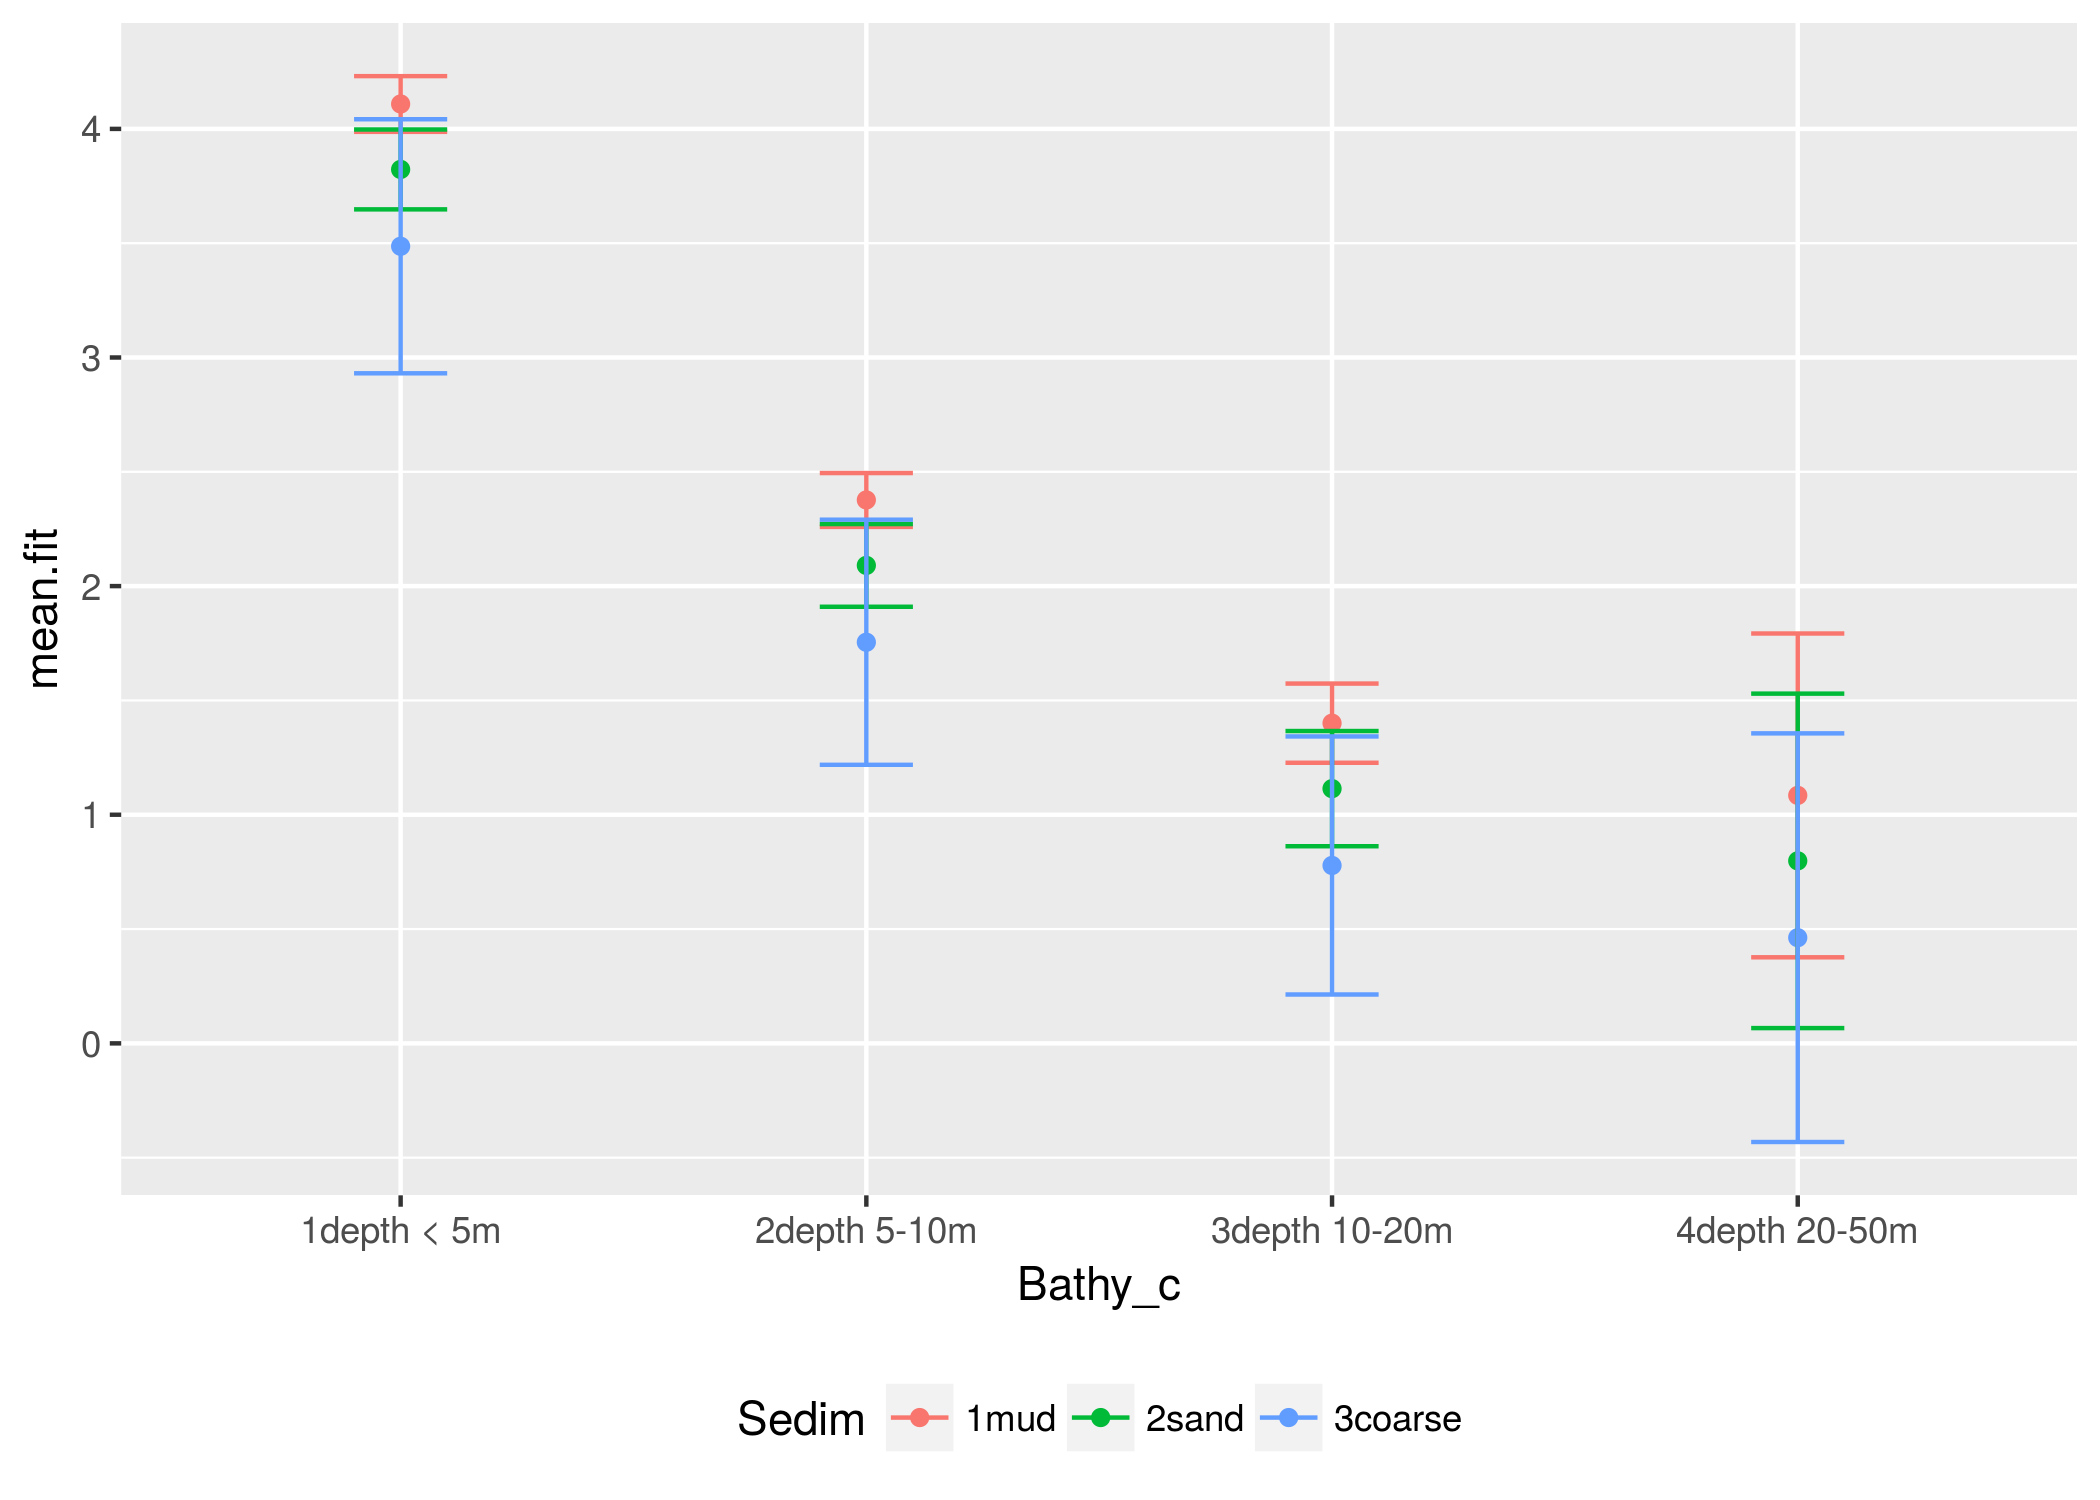
\includegraphics[width=0.8\linewidth]{FR_Quick_AllDataModel_Teacher_files/figure-latex/RFigGLMPredict-1} 

}

\caption{Prédictions du meilleur GLM sélectionné}\label{fig:RFigGLMPredict}
\end{figure}


\end{document}
